
% please use TexLive 2014 or later with the M&C macros freely
% available from tug.org or use any other recent version of LaTeX

\documentclass{book}

%the main style; default LibreCaslon font
\usepackage[raggedsec]{morgan2}
\usepackage{morgan-defs}

%to use Times New Roman, instead of LibreCaslon, please uncomment the next line
%\morgansetup{fontsetup=times}

% bibliography
\usepackage[square,comma,sort]{natbib}         % author-year
%usepackage[square,comma,sort,numbers]{natbib} % numbered

\setcounter{secnumdepth}{2}

\graphicspath{{./figures/}}     % folder for the figures in your book

\PassOptionsToPackage{hyphens}{url}
\usepackage[colorlinks=true,linkcolor=MyDarkBlue,
citecolor=MyDarkBlue,filecolor=MyDarkBlue,urlcolor=MyDarkBlue]{hyperref}

\renewcommand{\UrlBreaks}{\do\.\do\@\do\\\do\/\do\!\do\_\do\|\do\;\do\>\do\]%
\do\)\do\,\do\?\do\&\do\'\do+\do\=\do\#%
\do\a\do\b\do\c\do\d\do\e\do\f\do\g\do\h\do\i\do\j%
\do\k\do\l\do\m\do\n\do\o\do\p\do\q\do\r\do\s\do\t%
\do\u\do\v\do\w\do\x\do\y\do\z\do\A\do\B\do\C\do\D%
\do\E\do\F\do\G\do\H\do\I\do\J\do\K\do\L\do\M\do\N%
\do\O\do\P\do\Q\do\R\do\S\do\T\do\U\do\V\do\W\do\X%
\do\Y\do\Z}
\makeatletter
\g@addto@macro{\UrlBreaks}{\UrlOrds}
\renewcommand{\ALG@name}{\color{black}Algorithm}
\makeatother

%\makeindex                     % if you are creating an index for your book

\begin{document}

 \frontmatter                   % we'll produce the fm for you; 
    
\def\HALFTITLE{The Multifaceted Nature\\
			of Sustainability Challenges:\\
			An Engineering Perspective}
\def\TITLE{The Multifaceted Nature of Sustainability Challenges}
\def\AUTHORA{Jeremy Van Antwerp}
\def\AFFILIATIONA{Engineering Department, Calvin College}
\def\AUTHORB{Matthew Kuperus Heun}
\def\AFFILIATIONB{Engineering Department, Calvin College}
\def\AUTHORS{\AUTHORA\ and \AUTHORB}
\def\LECTURE{\ \#13}
\def\lcSYNTHESIS{Synthesis Lectures on XYZ}
\def\SYNTHESIS{\MakeUppercase{\textit{\lcSYNTHESIS}}}

\def\EDITOR{xxxx, \textit{yyyy}}


%%%%%%%%%%%% HALF TITLE PAGE 1-2

\thispagestyle{emptyrule}

\halftitle{\HALFTITLE}

\clearpage


%%%%%%%%%%%% FULL TITLE 5

\blankpage

\thispagestyle{emptyrule}
\title{\TITLE}

\vspace*{2pc}
\authorname{\AUTHORA}
\authoraffiliation{\AFFILIATIONA}

\vspace*{1pc}
\authorname{\AUTHORB}
\authoraffiliation{\AFFILIATIONB}

\vfill
\synthesis{\SYNTHESIS\LECTURE}
\morganlogo

\clearpage


%%%%%%%%%%%% ABSTRACT AND KEYWORDS   6

\thispagestyle{emptyrule}

\ABSTRACT
\noindent
The abstract goes here. 

The Abstract and the keywords have to fit in this page.
%end ABSTRACT

\keywords{%
xxx, yyyy, zz
}

\vfill

\clearpage


%%%%%%%%%%%%% DEDICATION  7-8


%{
%\clearpage
%\thispagestyle{plain}
%
%\vspace*{13pc}\Large\it
%\centerline{To Eric, Jacob, and my parents.}
%
%}
%
%\clearpage
 

%%%%%%%%%%%%%%%%%%%%%%%% TOC %%%%%%%%%%%%%%%%%%

%blankpage

{
\pagestyle{plain}
\tableofcontents
}

\clearpage
 
 
%%%%%%%%%%%%%%%%%%%%%%%% PREFACE %%%%%%%%%%%%%%%%%%%
 
 
\blankpage

{
\chapter*{Preface}
\addcontentsline{toc}{chapter}{\protect\numberline{}{Preface}}
\thispagestyle{plain}
\markboth{PREFACE}{PREFACE}

\noindent
This is the Preface.


\vspace*{2pc}
\noindent\AUTHORS\\
\noindent December 2019
}

\clearpage


%%%%%%%%%%%%%%%%%%%%%%%% ACK %%%%%%%%%%%%%%%%%%%


\blankpage

\chapter*{Acknowledgments}
\addcontentsline{toc}{chapter}{\protect\numberline{}{Acknowledgments}}
\thispagestyle{plain}
\markboth{ACKNOWLEDGMENTS}{ACKNOWLEDGMENTS}

\noindent
This the Acknowledgments' page.

\vspace*{2pc}
\noindent\AUTHORS\\
\noindent December 2019
 
\clearpage

\blankpage

                  % we'll need an Abstract and Keywords
								% please see the abs-pref folder for some pdf examples

 \mainmatter                    % sample chapters
    
\chapter{Information Theory and Rate Distortion Theory}
\label{ch01}


Please see below examples of equations using \verb+\begin{equation}+ \ldots
\verb+\end{equation}+ and \verb+align+.

The M\&C macros support various environments like:
constraint, construction, 
convention, conventions, corollary, definition, dictionary,
example, lemma, note, notation, observation, property, proposition,
remark, rules, theorem, etc.

What if you need an environment that the macros do not provide,
like ``guesswork?'' You create it with \verb+newMCtheorem+:

\verb+newMCtheorem}{guesswork}{GuessWork}+

\newMCtheorem{guesswork}{GuessWork}

\noindent
and use then use it:
\begin{guesswork}
This is pure guess work.
\end{guesswork}


\section{Introduction}
\label{ch01.sec1}

Thus far in the book, the term \textit{information}
\index{information}%
has been used sparingly and when
it has been used, we have purposely been imprecise as to its meaning.

\begin{figure}[hbt] % 01
\centering
  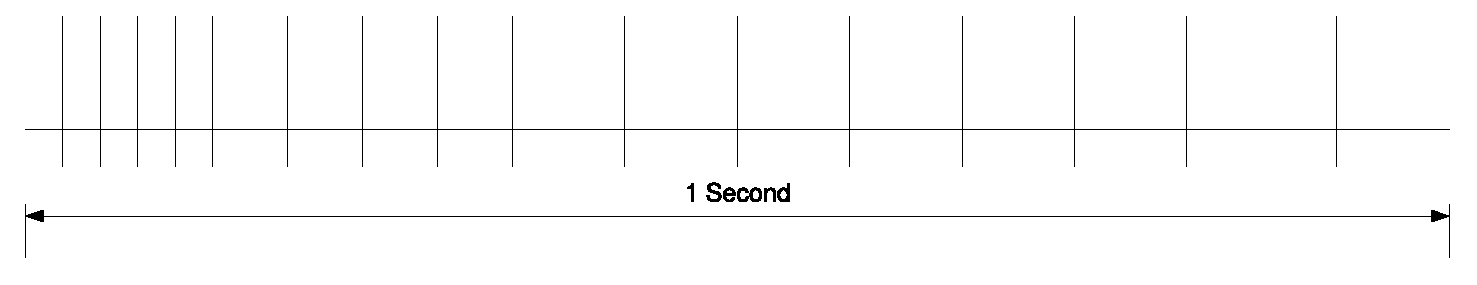
\includegraphics[width=3.3in]{line-spaces.eps}
\caption{Communication system block diagram.}
\label{ch01.fig1} 
\end{figure}

\begin{figure}[hbt] % 01
\centering
  \figboxes
\caption{Communication system block diagram.}
\label{ch01.fig2} 
\end{figure}

Examples of side-by-side figures.

%  F 2
\begin{figure}[hbt]%
\centering
\begin{subfigure}[t]{0.45\textwidth}%
	\smfigboxes
\caption{Annotated visualization of the structure of a biological neuron, reconstructed from electron microscope images of 30nm-thick slices of a mouse 
brain~\cite{tesniere59}.}%
\label{fig:bioneuron}%
\end{subfigure}%
\qquad%
\begin{subfigure}[t]{0.45\textwidth}%
	\smfigboxes
\caption{The shape of an action potential. A small external voltage stimulus (blue) triggers a cascade of charge build-up inside a neuron (red) via voltage-gated ion channels. The activation threshold is shown as a dotted line. Simulated using a Hodgkin-Huxley model of a neuron~\protect\cite{weber-97}.}%
\label{fig:ap}%
\end{subfigure}%
\caption{The structure and operation of biological neurons.}%
\end{figure}

%  F 3
\begin{figure}[b]
\centering
\begin{subfigure}[t]{0.45\textwidth}
	\smfigboxes
\caption{Points in $\mathbb{R}^2$, subdivided by a single linear classifier. One simple way of understanding linear classifiers is as a line (or hyper-plane, in higher dimensions) which splits space into two regions. In this example, points above the line are mapped to class 1 (red); those below, to class 0 (blue).}
\label{subfig:linclass}
\end{subfigure}%
\qquad%
\begin{subfigure}[t]{0.45\textwidth}
	\smfigboxes
\caption{Points in $\mathbb{R}^2$, subdivided by a combination of four linear classifiers. Each classifier maps \emph{all} points to class 0 or 1, and an additional linear classifier is used to combine the four. This hierarchical model is strictly more expressive than any linear classifier by itself.}
\label{subfig:circclass}
\end{subfigure}%
\caption{Simple elements can be combined to express more complex relationships.
This is one basic tenet of deep neural networks.}
\label{fig:classifiers}
\end{figure}


\section{Entropy and Average Mutual Information}
\label{ch01.sec2}

Consider a discrete random variable $U$ that takes on
the values $\{u_1, u_2, \dots, u_M\}$, where the set of possible
values of $U$ is often called the \textit{alphabet} and the elements
of the set are called \textit{letters} of the alphabet. Let $P_U(u)$
denote the probability  assignment  over the alphabet, then we can
define the \textit{self-information} of the event $ u = u_j $ by
\begin{equation}
  I_U \left( u_j \right) = \log \frac{1}{P_U (u_j)} = - \log P_U
    \left( u_j \right).
\label{ch01.eq1}
\end{equation}

\begin{example}
\label{ch01.ex1}
Given a random variable $U$ with four equally likely letters
in its alphabet, we wish to find $H(U)$. Clearly, $M=4$
and $P_U(u_i)= \tfrac{1}{4}$ for $ i = 1, 2, 3, 4 $.

\begin{align}
    I_{W;X}\left(w_j;x_k\right)
    & = \log
    \frac{P_{WX}\left(w_j, x_k\right)}{P_W\left(w_j\right)
              P_X\left(x_k\right)}
    \notag\\
    & = \log
    \frac{P_{X|W} \left( x_k | w_j\right)} {P_X \left(x_k\right)}
    =
     I_{X;W} \left(x_k; w_j\right).
\label{ch01.eq2}
\end{align}
\end{example}

\begin{property}
\label{ch01.pro1}
Let $U$ be a random variable with possible values $\{u_1,u_2,\dots, u_M\}$.
\end{property}

Example~\ref{ch01.ex1} illustrates Property~\ref{ch01.pro1}.

\begin{property}
\label{ch01.pro2}
Let $W$ and $X$ be jointly distributed random variables.
\end{property}

\begin{example}
\label{ch01.ex2}
Here we wish to calculate the mutual information and the average
mutual information for the probability assignments
(with $M=2$ and $N=2$)
\begin{equation}
 P_W \big(w_1\big) = P_W \big(w_2\big) = \tfrac{1}{2}
\label{ch01.eq3}
\end{equation}
\end{example}

\begin{example}[\cite{Boeringer}]
\label{ch01.ex3}
The source output is a ternary-valued random variable that takes on the
values $\{ u_1, u_2, u_3 \}$ with probabilities
$P(u_1) = 0.7, P(u_2) = 0.15 = P(u_3)$. 
\end{example}

\begin{theorem}[(Source Coding Theorem).]
\label{ch01.th1}
For a DMS with entropy $H(U)$,
the minimum average codeword length per source letter $(\bar{n})$ for any
code is lower
bounded by $H(U)$, that is, $\bar{n} \geq H(U)$, and further, $\bar{n}$
can be made as close to $H(U)$
as desired for some suitably chosen code.
\end{theorem}

\begin{theorem}[(Channel Coding Theorem~\cite{Wen-ChungLiu2005}).]
\label{ch01.th2}
Given a DMS
with entropy $H$ bits/source letter and a DMC with capacity $C$
bits/source letter,
if $H \leq C$, the source output can be encoded for transmission over
the channel with
an arbitrarily small bit error probability. Further, if $H > C$, the bit error
probability is bounded away from $0$.
\end{theorem}

\begin{proof}
This result can be proved in several ways, including calculus of
variations~\cite{WenWangetal2005} inequality; however, an
alternative method is used here.
\end{proof}

\begin{table}[hbt]
\caption{Timer0 Compare Output Mode, non-PWM Mode}
\label{ch01.tab1} 
\begin{center}
\begin{tabular}{|c|l|}
    \cb COM0x1-0
  & \cb Description 
\\
    \cw 00
  & \cw Normal port operation
\\
    \cy 01
  & \cy Toggle on Compare Match
\\
    \cw 10
  & \cw Clear on Compare Match
\\
    \cy 11
  & \cy Set on Compare Match
\\
\hline
\end{tabular}
\end{center}
\end{table}


\begin{center}
\begin{tabular}{|cl|}
    \cb COM0x1-0
  & \cb Description 
\\
    \cw 00
  & \cw Normal port operation
\\
    \cy 01
  & \cy Toggle on Compare Match
\\
    \cw 10
  & \cw Clear on Compare Match
\\
    \cy 11
  & \cy Set on Compare Match
\\
\hline
\end{tabular}
\end{center}


\section*{Summary}

In this chapter we have discussed very briefly some of the salient
results from information theory and rate distortion theory and have
indicated how these results can be used to bound communication system
performance.


\section*{Problems}
\index{problems}%

\begin{problems}

\item
A random variable $U$ has a sample space consisting of the set
of all possible binary sequences of length $N$, denoted
$\{u_j, j=1, 2, \ldots, 2^N \}$.

\item
Given a random variable $U$ with the alphabet $\{ u_1, u_2, u_3, u_4 \}$
and probability assignments $P(u_1) = 0.8, P(u_2)=0.1$,
$P(u_3) = 0.05, P(u_4)=0.05$, calculate the entropy of $U$.
Compare your result to a random variable with equally likely values.

\end{problems}

\clearpage

                % various environments like theorem,
    
%blankpage

\chapter{Jordan Canonical Form}
\label{ch02}
\index{jordan canonical form@Jordan Canonical Form}%

\section{The Diagonalizable Case}

Although, for simplicity, most of our examples
will be over the real numbers
(and indeed over the rational numbers), we will consider that
\textit{all of our vectors and matrices
are defined over the complex numbers} $\mathbb{C}$.
It is only with this assumption that the
theory of Jordan Canonical Form (JCF) works
\index{jcf@JCF}%
completely.
See Remark~\ref{ch02.rem1} for the key reason why.

\begin{definition}
\label{ch02.def1}
If \(v \neq 0\) is a vector such that, for some
$\lambda$,
\[
A v = \lambda v,
\]
then $v$ is an \textit{eigenvector} of $A$ associated
\index{eigenvector}%
to the \textit{eigenvalue} $\lambda$.
\index{eigenvalue}%
\end{definition}

\begin{example}
\label{ch02.ex1}
Let $A$ be the matrix $A =$
Then, as you can check, if $v_1 =$ 
then $A v_1 = 3 v_1$, so $v_1$ is an eigenvector of $A$ with associated
eigenvalue $3$, and if $v_2 =$ 
then $A v_2 = -2 v_2$, so $v_2$ is
an eigenvector of $A$ with associated eigenvalue $-2$.
\end{example}

\begin{remark}
\label{ch02.rem1}
This is the customary definition of the characteristic
\index{characteristic polynomial}%
polynomial.
But note that, if $A$ is an $n$-by-$n$ matrix, then the matrix
$\lambda I - A$ is obtained from the matrix $A - \lambda I$ by multiplying
each of its $n$ rows by $-1$, and hence
In practice, it is most convenient
to work with $A -\lambda I$ in finding eigenvectors---this minimizes
arithmetic---and when we come to find
chains of generalized eigenvectors in
Section~1.2,
it is (almost) essential to use $A -\lambda I$, as using
$\lambda I - A$ would introduce lots of spurious minus signs.
\end{remark}

\clearpage

                % example, etc.
    
%blankpage

\chapter{An Algorithm}
\label{ch03}

The navigation oriented heuristic ($h3$) considers the site topology.
Accesses to cached pages are not recorded in the
Web log due to the browser or proxy cache.
Therefore, references to those pages are missed.
The missing references in the log file can be found using a set of
assumptions.
The referrer field of the Web log or the Web site structure can be used
to infer cached pages.
If a requested Web page $p_i$ is not reachable
from previously visited pages in a
session, then a new session is constructed starting with page $p_i$.

\begin{algorithm}
\hrulefill

 \textit{Input :} Web server logs \newline
 \textit {Output :} set of user sessions
$\mathcal{S}=\{s_{1},...,s_{M}\}$

\hrulefill

\begin{algorithmic}[1]
 \STATE $\mathcal{S}=\{\emptyset\}$
 \STATE Order all Web logs by user IDs ($u_k$) and time increasingly
 \FORALL {user ID $u_k$}
    \STATE Create a new user session in $\mathcal{S}$ for user $u_k$
    \FOR {i=1 to the number of records of this $u_k$}
    	\IF {$t_{i+1} - t_i < \triangle t$}
    		\STATE insert this record into user session
    	\ELSE
    		\STATE Create a new user session in $\mathcal{S}$ for user $u_k$
    	\ENDIF
    \ENDFOR
 \ENDFOR
\end{algorithmic}
\hrulefill
 \caption{Construction of user sessions from Web server logs using $h1$
 heuristic}
\label{alg:visitingTimeAlg}
\end{algorithm}

\clearpage

                % algorithm sample
    
%blankpage

\chapter{Shaded Areas}
\label{ch04}

M\&C provides a macro called \verb+mcframe+ that allows us to
create a frame around some text which automatically breaks its contents
across pages. 

\verb+\begin{mcframe}[width](text-width)<background-color>+\\

\ldots

\verb+\end{mcframe}+

The optional arguments are:
\begin{itemize}
\item
\verb+width+ defaults to the width of the page
\item
\verb+text-width+ defaults to an indent of 10pt in each margin
\item
\verb+background-color+ defaults to the \verb+bluetwenty+ color of the
	M\&C books.
\end{itemize}

\blankline
Here are a few examples using some text from the book \textit{General Game 
Playing} by M. Genesereth and M. Thielscher that was published by M\&C in 
March, 2014:

\begin{mcframe}
\verb+\begin{mcframe}+\\
Games of strategy, such as Chess, couple intellectual activity with
competition.
We can exercise and improve our intellectual skills by playing such games.
The competition adds excitement and allows us to
compare our skills to those of others.
The same motivation accounts for
interest in Computer Game Playing as a testbed for Artificial Intelligence.
Programs that think better should be able to win more
games, and so we can use competitions as an evaluation technique for
intelligent systems.

Unfortunately, building programs to play specific games has limited
value in AI.  (1)~To begin with, specialized game players are very narrow.
They can be good at one game but not another. Deep Blue may have beaten
the world Chess champion, but it has no clue how to play checkers.  (2)~A
second problem with specialized game playing systems is that they do only
part of the work. Most of the interesting analysis and design is done in
advance by their programmers. The systems themselves might as well be
tele-operated.

All is not lost. The idea of game playing can be used to good effect
to inspire and evaluate good work in Artificial Intelligence, but it
requires moving more of the design work to the computer itself.
This can be done by focussing attention on General Game Playing.\\
\verb+\end{mcframe}+
\end{mcframe}

\begin{mcframe}[.7\textwidth](.6\textwidth)
\verb+\begin{mcframe}[.7\textwidth](.6\textwidth)+\\
Games of strategy, such as Chess, couple intellectual activity with
competition.
We can exercise and improve our intellectual skills by playing such games.
The competition adds excitement and allows us to
compare our skills to those of others.
The same motivation accounts for
interest in Computer Game Playing as a testbed for Artificial Intelligence.
Programs that think better should be able to win more
games, and so we can use competitions as an evaluation technique for
intelligent systems.

Unfortunately, building programs to play specific games has limited
value in AI.  (1)~To begin with, specialized game players are very narrow.
They can be good at one game but not another. Deep Blue may have beaten
the world Chess champion, but it has no clue how to play checkers.  (2)~A
second problem with specialized game playing systems is that they do only
part of the work. Most of the interesting analysis and design is done in
advance by their programmers. The systems themselves might as well be
tele-operated.\\
\verb+\end{mcframe}+
\end{mcframe}

\begin{mcframe}[.8\textwidth](.7\textwidth)<green>
\verb+\begin{mcframe}[.8\textwidth](.7\textwidth)<green>+\\
Games of strategy, such as Chess, couple intellectual activity with
competition.
We can exercise and improve our intellectual skills by playing such games.
The competition adds excitement and allows us to
compare our skills to those of others.
The same motivation accounts for
interest in Computer Game Playing as a testbed for Artificial Intelligence.
Programs that think better should be able to win more
games, and so we can use competitions as an evaluation technique for
intelligent systems.

Unfortunately, building programs to play specific games has limited
value in AI.  (1)~To begin with, specialized game players are very narrow.
They can be good at one game but not another. Deep Blue may have beaten
the world Chess champion, but it has no clue how to play checkers.  (2)~A
second problem with specialized game playing systems is that they do only
part of the work. Most of the interesting analysis and design is done in
advance by their programmers. The systems themselves might as well be
tele-operated.\\
\verb+\end{mcframe}+
\end{mcframe}

\clearpage

                % shaded blocks in your pages
    
%blankpage

\chapter{Math}
\label{ch05}

\section{Bold Math}
Sometimes you have a math symbol in bold to indicate, for example,
a vector or special functions. Use \verb+\mathbf{x}+ for letters
and \verb+\bm{\Phi}+ for Greek letters.

\noindent
\ldots
$\bm{\Phi}$ and $\bm{\Theta}$ are the distribution functions
governing the likelihood of $\mathcal{X}$ and $\mathbf{Z}$ \ldots

\blankline
Some notes:
\begin{itemize}
\item
use \verb+\bm{\Phi}+ to produce a bold Greek symbol Phi.
\item
use \verb+\mathcal{X}+ to display the caligraphic letter X
\item
use \verb+\mathbf{Z}+ to dispaly bold non-Greek symbols
\end{itemize}

\blankline
If you plan to use Greek symbols to identify, for example, vectors, you could
create a macro, like

\verb+\newcommand{\vect}[1]{\bm{#1}}+

\newcommand{\vect}[1]{\bm{#1}}

and then use

\noindent
\begin{verbatim}
\ldots the vectors are $\vect{\Phi}$ and $\vect{\Theta}$ \ldots
\end{verbatim}

to produce

\noindent
\ldots the vectors are $\vect{\Phi}$ and $\vect{\Theta}$ \ldots

\blankline
The idea is to have macro names for different constructs.
If you chose to use a different representation for vectors,
you change the macro and rerun your manuscript.


\section{Math Variables}

When we have a math variable with more than one character,
like \textit{abcd}, \LaTeX{} treats each character as a separate variable.
With Caslon fonts, that we use to produce your book, that space is noticeable.

We eliminat the extra space using \verb+\mathit+:

\verb+\mathit{abcd} = 3.+
$$
\mathit{abcd} = 3.
$$

If we use the variable \textit{abcd} often, as in

\verb|\mathit{abcd} = \mathit{abcd}^2 - \sqrt{\mathit{abcd}} + \mathit{abcd},|

$$
\mathit{abcd} = \mathit{abcd}^2 - \sqrt{\mathit{abcd}} + \mathit{abcd},
$$
we can create a separate macro for the variable:

\verb+\newcommand{\abcd}{\mathit{abcd}}+
\newcommand{\abcd}{\mathit{abcd}}

\noindent
Then we can use \verb+\abcd+ in the expressions:

\verb|\abcd = \abcd^2 - \sqrt{\abcd} + \abcd,|

$$
\abcd = \abcd^2 - \sqrt{\abcd} + \abcd,
$$

If there is already a predefined command with the same name,
we use instead something like \verb+Abcd+:

\verb+\newcommand{\Abcd}{\mathit{abcd}}+
\newcommand{\Abcd}{\mathit{abcd}}

\noindent
Then we can use \verb+\Abcd+ in the expressions:

\verb|\Abcd = \Abcd^2 - \sqrt{\Abcd} + \Abcd.|

$$
\Abcd = \Abcd^2 - \sqrt{\Abcd} + \Abcd.
$$


\clearpage

                % bold math and math variables
    
%blankpage

\chapter{Citations with Author-Year}
\label{ch06}

An alternative to numerical \LaTeX\ citations makes reference to published
works by citing the author's name and year of publication. The entries in 
the bibliographic listing are not numbered. The citation itself may be 
either parenthetical like \citep{carroll98} or textual as shown by
\citet{carroll98}.

The \verb+natbib+ package by Patrick W. Daly is the most universal package
for Author-Year citation and it is compatible with \verb+\bibitem+ syntaxes
and with the \verb+.bst+ files of author-year packages such as
\verb+apalike+, \verb+chicago+, and \verb+harvard+.

If you create a bibliography by hand, please see the file \verb+biblio.tex+
in the \verb+latex+ directory of \verb+bib-AY.zip+.
The \verb+biblio.tex+ files shows the syntax that \verb+natbib.sty+ 
requires and notice how we use
that package in~\verb+book.tex+ and in~\verb+ch01.tex+. 
You can find the details about \verb+natbib+ and Author-Year bibliographies
in~\citet[pages~218-221]{KD:2004}.

Note that we have bibliographic references like \verb+carroll98+,
\verb+KD:2004+, and \verb+weber-97+. Pick a style that works for you
and stay with it, then it will be easier for yourself and others to 
maintain and modify your bibliography and citations.

If you use \verb+.bib+ files then you should know about \verb+BibTeX+,
\verb+.bst+ files, and you should know how to create the \verb+.bbl+
files as well.
(If you use \verb+.bib+ files but you do not know the rest, you should
consult a local expert before continuing with \verb+.bib+ or create
your bibliography by hand.)
If you know the steps we mentioned above and you wish to create an 
Author-Year bibliography and citations, then you are in luck: 
there are three \verb+.bst+ that are provided with \verb+natbib+.
They are: \verb+plainnat+, \verb+unsrtnat+, and \verb+abbrvnat+.

Once you create your \verb+.bbl+ file(s), please submit them along with
your manuscript files, style files, and (preferably) \verb+.eps+ figures with 
\verb+BoundingBox+es to \textit{Morgan and Claypool Publishers.}

You can get a free copy of the \verb+natbib+ package  from CTAN at
\begin{center}
\verb+http://www.ctan.org/tex-archive/macros/latex/contrib/natbib/+
\end{center}
and download the file \verb+natbib.zip+.

Here are some more samples using the citations that appear in the file
\verb+biblio.tex+ that we built by hand.

The next paragraph uses text citations using \verb+\citet+ (cite as text):\\
\noindent
There are several textbooks that give a general 
introduction to dependency grammar but
most of them in other languages than English, for example,
\citet{tarvainen82} and~\citet{weber-97}.

The last paragraph uses text citations with parentheses
using \verb+\citetp+:\\
\noindent
Tesni{\`e}re's seminal work was published
posthumously as~\citep{tesniere59}. 
Other influential theories in the dependency
grammar tradition include Functional Generative
Description~\citep{SHP:1986}.

Please see the bibliography on the next page and the file \verb+biblio.tex+.

\clearpage

                % bibliography using Author-Year

    
\blankpage

\begin{thebibliography}{xx}
\addcontentsline{toc}{chapter}{\protect\numberline{}{Bibliography}}
\markboth{BIBLIOGRAPHY}{BIBLIOGRAPHY}

\bibitem[Boeringer and Werner(2004)D. Boeringer and D. Werner]{Boeringer}
D. Boeringer and D. Werner,
``Particle swarm optimization versus genetic algorithms for
phased array synthesis,''
\textit{IEEE Trans. Antennas Propagat.,}
vol.~52, no.~3, pp.~771--779, 2004.

\bibitem[Carroll et~al.(1998)Carroll, Briscoe, and Sanfilippo]{carroll98}
Carroll, John, Briscoe, Edward, and Sanfilippo, Antonio
Supertagging: An approach to almost parsing,
\textit{Computational Linguistics} 25(2):237--267.

\bibitem[Ho et al(2005)Ho et al]{Hoetal2005}
S. Ho, S. Yang, G. Ni, E. W. C. Lo, and H. C. Wong,
``A particle swarm optimization-based method for multiobjective
design optimizations,''
\textit{IEEE Trans. Magn.},
vol.~41, no.~5, pp.~1756--1759, 2005.

\bibitem[Kopka and Daly(2004)W. Kopka and P.W. Daly]{KD:2004}
Kopka, Helmut and Daly, Patrick W. 
\textit{Guide to \LaTeX,} fourth edition, Addison Wesley.

\bibitem[Levin (2002)F.S. Levin]{Levin2002}
F. S. Levin,
\textit{An Introduction to Quantum Theory},
Cambridge: Cambridge University Press, 2002.

\bibitem[Liu (2005)W.-C. Liu]{Wen-ChungLiu2005}
W-C Liu,
``A design of a multiband
CPW-fed monopole antenna using a particle swarm optimization approach,''
\textit{IEEE Trans. Antennas Propagat.,}
vol.~53, no.~10, pp.~3273--3279, 2005.

\bibitem[Sgall et~al.(1986)Sgall, Haji\v{c}ov\'{a}, and Panevov\'{a}]
{SHP:1986}
Sgall, Petr, Haji\v{c}ov\'{a}, Eva, and Panevov\'{a}, Jarmila.
\textit{The Meaning of the Sentence in Its Pragmatic Aspects}, Reidel.

\bibitem[Tarvainen (1982)Tarvainen]{tarvainen82}
Tarvainen, Kalevi.  
\textit{Einf\"{u}hrung in die {D}ependenzgrammatik}, Niemeyer.

\bibitem[Tesni{\`e}re (1959)Tesni{\`e}re]{tesniere59}
Tesni{\`e}re, Lucien.  
\textit{\'El\'ements de syntaxe structurale}, Editions Klincksieck.

\bibitem[Weber (1997)Weber, H.J.]{weber-97}
Weber, H.~J. 
\textit{Dependenzgrammatik.\ Ein interaktives Arbeitsbuch},
G\"unter Narr.

\bibitem[Wang et al(2005)W. Wang et al]{WenWangetal2005}
W. Wang, Y. Lu, J. S. Fu, and Y. Z. Xiong,
``Particle swarm optimization and finite-element based
approach for microwave filter design,''
\textit{IEEE Trans. Magn.},
vol.~41, no.~5, pp.~1800--1803, 2005.

\end{thebibliography}

\clearpage

              % bibliography

 \backmatter                    % back matter
    
%blankpage

\chapter*{Author's Biography}
\markboth{AUTHOR'S BIOGRAPHY}{AUTHOR'S BIOGRAPHY}
\addcontentsline{toc}{chapter}{\protect\numberline{}{Author's Biography}}


\section*{Jeremy Van Antwerp}

% Adjust spacing so the photo looks nice in the paragraph.
\setlength{\intextsep}{-7pt}%
\setlength{\columnsep}{8pt}%
\begin{wrapfigure}{L}{0.25\textwidth}
  \begin{center}
    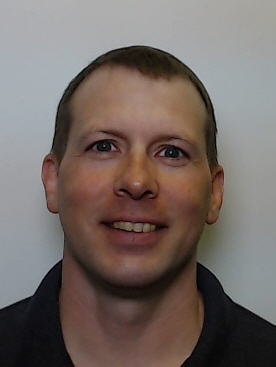
\includegraphics[width=0.25\textwidth]{figures/jva-headshop.jpeg}
  \end{center}
\end{wrapfigure}
\textbf{Jeremy Van Antwerp} earned a Ph.D.\ in chemical engineering from 
the University of Illinois at Urbana-Champaign.
More text here.
More text here.
More text here.
More text here.
More text here.
More text here.
More text here.
More text here.
More text here.
More text here.
More text here.
More text here.
More text here.
More text here.
More text here.
More text here.
More text here.
More text here.
More text here.
More text here.
More text here.
More text here.
More text here.
More text here.
More text here.
More text here.
More text here.
More text here.
More text here.
More text here.
More text here.
More text here.
More text here.
More text here.
More text here.
More text here.
More text here.
More text here.
More text here.
More text here.
More text here.
More text here.
More text here.
More text here.
More text here.
More text here.
More text here.
More text here.
More text here.


\section*{Matthew Kuperus Heun}

% Adjust spacing so the photo looks nice in the paragraph.
\setlength{\intextsep}{-7pt}%
\setlength{\columnsep}{8pt}%
\begin{wrapfigure}{L}{0.25\textwidth}
  \begin{center}
    \includegraphics[width=0.25\textwidth]{figures/Heun-pub-photo-headshot}
  \end{center}
\end{wrapfigure}
\textbf{Matthew Kuperus Heun} is Professor of Engineering 
(mechanical concentration)
at Calvin College in Grand Rapids, MI, USA.
He earned an M.S.\ and Ph.D.\ in mechanical engineering from 
the University of Illinois at Urbana-Champaign and 
later worked at NASA's Jet Propulsion Laboratory and at Global Aerospace Corporation. 
He has been a visiting scholar at the Centre for Renewable and Sustainable Energy Studies 
at the University of Stellenbosch, South Africa. 
His long-term research question is 
``What is the relationship between energy and the economy when viewed through the lens of sustainability?''
In addition to scores of articles, he is lead author of 
\emph{Beyond GDP: National accounting in the age of resource depletion}~\citep{Heun:2015aa} 
and a co-editor of
\emph{Beyond Stewardship: New approaches to creation care}~\citep{Warners:2019aa}.
                 % author(s)'s short bio(s)
								% please see the bios folder for some pdf examples

%   
% please use TexLive 2014 or later with the M&C macros freely
% available from tug.org or use any other recent version of LaTeX

\documentclass{book}

%the main style; default LibreCaslon font
\usepackage[raggedsec]{morgan2}
\usepackage{morgan-defs}

%to use Times New Roman, instead of LibreCaslon, please uncomment the next line
%\morgansetup{fontsetup=times}

% bibliography
\usepackage[square,comma,sort]{natbib}         % author-year
%usepackage[square,comma,sort,numbers]{natbib} % numbered

\setcounter{secnumdepth}{2}

\graphicspath{{./figures/}}     % folder for the figures in your book

\PassOptionsToPackage{hyphens}{url}
\usepackage[colorlinks=true,linkcolor=MyDarkBlue,
citecolor=MyDarkBlue,filecolor=MyDarkBlue,urlcolor=MyDarkBlue]{hyperref}

\renewcommand{\UrlBreaks}{\do\.\do\@\do\\\do\/\do\!\do\_\do\|\do\;\do\>\do\]%
\do\)\do\,\do\?\do\&\do\'\do+\do\=\do\#%
\do\a\do\b\do\c\do\d\do\e\do\f\do\g\do\h\do\i\do\j%
\do\k\do\l\do\m\do\n\do\o\do\p\do\q\do\r\do\s\do\t%
\do\u\do\v\do\w\do\x\do\y\do\z\do\A\do\B\do\C\do\D%
\do\E\do\F\do\G\do\H\do\I\do\J\do\K\do\L\do\M\do\N%
\do\O\do\P\do\Q\do\R\do\S\do\T\do\U\do\V\do\W\do\X%
\do\Y\do\Z}
\makeatletter
\g@addto@macro{\UrlBreaks}{\UrlOrds}
\renewcommand{\ALG@name}{\color{black}Algorithm}
\makeatother

% Begin packages imported by the authors.
\usepackage{wrapfig}  % To wrap text around figures.



%\makeindex                     % if you are creating an index for your book

\begin{document}

 \frontmatter                   % we'll produce the fm for you; 
    
\def\HALFTITLE{The Multifaceted Nature\\
			of Sustainability Challenges:\\
			An Engineering Perspective}
\def\TITLE{The Multifaceted Nature of Sustainability Challenges}
\def\AUTHORA{Jeremy Van Antwerp}
\def\AFFILIATIONA{Engineering Department, Calvin College}
\def\AUTHORB{Matthew Kuperus Heun}
\def\AFFILIATIONB{Engineering Department, Calvin College}
\def\AUTHORS{\AUTHORA\ and \AUTHORB}
\def\LECTURE{\ \#13}
\def\lcSYNTHESIS{Synthesis Lectures on XYZ}
\def\SYNTHESIS{\MakeUppercase{\textit{\lcSYNTHESIS}}}

\def\EDITOR{xxxx, \textit{yyyy}}


%%%%%%%%%%%% HALF TITLE PAGE 1-2

\thispagestyle{emptyrule}

\halftitle{\HALFTITLE}

\clearpage


%%%%%%%%%%%% FULL TITLE 5

\blankpage

\thispagestyle{emptyrule}
\title{\TITLE}

\vspace*{2pc}
\authorname{\AUTHORA}
\authoraffiliation{\AFFILIATIONA}

\vspace*{1pc}
\authorname{\AUTHORB}
\authoraffiliation{\AFFILIATIONB}

\vfill
\synthesis{\SYNTHESIS\LECTURE}
\morganlogo

\clearpage


%%%%%%%%%%%% ABSTRACT AND KEYWORDS   6

\thispagestyle{emptyrule}

\ABSTRACT
\noindent
The abstract goes here. 

The Abstract and the keywords have to fit in this page.
%end ABSTRACT

\keywords{%
xxx, yyyy, zz
}

\vfill

\clearpage


%%%%%%%%%%%%% DEDICATION  7-8


%{
%\clearpage
%\thispagestyle{plain}
%
%\vspace*{13pc}\Large\it
%\centerline{To Eric, Jacob, and my parents.}
%
%}
%
%\clearpage
 

%%%%%%%%%%%%%%%%%%%%%%%% TOC %%%%%%%%%%%%%%%%%%

%blankpage

{
\pagestyle{plain}
\tableofcontents
}

\clearpage
 
 
%%%%%%%%%%%%%%%%%%%%%%%% PREFACE %%%%%%%%%%%%%%%%%%%
 
 
\blankpage

{
\chapter*{Preface}
\addcontentsline{toc}{chapter}{\protect\numberline{}{Preface}}
\thispagestyle{plain}
\markboth{PREFACE}{PREFACE}

\noindent
This is the Preface.


\vspace*{2pc}
\noindent\AUTHORS\\
\noindent December 2019
}

\clearpage


%%%%%%%%%%%%%%%%%%%%%%%% ACK %%%%%%%%%%%%%%%%%%%


\blankpage

\chapter*{Acknowledgments}
\addcontentsline{toc}{chapter}{\protect\numberline{}{Acknowledgments}}
\thispagestyle{plain}
\markboth{ACKNOWLEDGMENTS}{ACKNOWLEDGMENTS}

\noindent
This the Acknowledgments' page.

\vspace*{2pc}
\noindent\AUTHORS\\
\noindent December 2019
 
\clearpage

\blankpage

                  % we'll need an Abstract and Keywords
								% please see the abs-pref folder for some pdf examples

 \mainmatter                    % sample chapters
    
\chapter{Information Theory and Rate Distortion Theory}
\label{ch01}


Please see below examples of equations using \verb+\begin{equation}+ \ldots
\verb+\end{equation}+ and \verb+align+.

The M\&C macros support various environments like:
constraint, construction, 
convention, conventions, corollary, definition, dictionary,
example, lemma, note, notation, observation, property, proposition,
remark, rules, theorem, etc.

What if you need an environment that the macros do not provide,
like ``guesswork?'' You create it with \verb+newMCtheorem+:

\verb+newMCtheorem}{guesswork}{GuessWork}+

\newMCtheorem{guesswork}{GuessWork}

\noindent
and use then use it:
\begin{guesswork}
This is pure guess work.
\end{guesswork}


\section{Introduction}
\label{ch01.sec1}

Thus far in the book, the term \textit{information}
\index{information}%
has been used sparingly and when
it has been used, we have purposely been imprecise as to its meaning.

\begin{figure}[hbt] % 01
\centering
  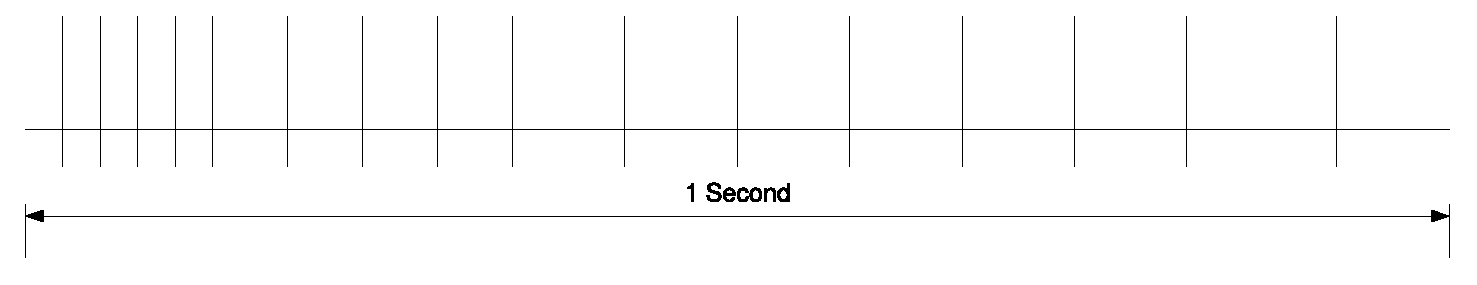
\includegraphics[width=3.3in]{line-spaces.eps}
\caption{Communication system block diagram.}
\label{ch01.fig1} 
\end{figure}

\begin{figure}[hbt] % 01
\centering
  \figboxes
\caption{Communication system block diagram.}
\label{ch01.fig2} 
\end{figure}

Examples of side-by-side figures.

%  F 2
\begin{figure}[hbt]%
\centering
\begin{subfigure}[t]{0.45\textwidth}%
	\smfigboxes
\caption{Annotated visualization of the structure of a biological neuron, reconstructed from electron microscope images of 30nm-thick slices of a mouse 
brain~\cite{tesniere59}.}%
\label{fig:bioneuron}%
\end{subfigure}%
\qquad%
\begin{subfigure}[t]{0.45\textwidth}%
	\smfigboxes
\caption{The shape of an action potential. A small external voltage stimulus (blue) triggers a cascade of charge build-up inside a neuron (red) via voltage-gated ion channels. The activation threshold is shown as a dotted line. Simulated using a Hodgkin-Huxley model of a neuron~\protect\cite{weber-97}.}%
\label{fig:ap}%
\end{subfigure}%
\caption{The structure and operation of biological neurons.}%
\end{figure}

%  F 3
\begin{figure}[b]
\centering
\begin{subfigure}[t]{0.45\textwidth}
	\smfigboxes
\caption{Points in $\mathbb{R}^2$, subdivided by a single linear classifier. One simple way of understanding linear classifiers is as a line (or hyper-plane, in higher dimensions) which splits space into two regions. In this example, points above the line are mapped to class 1 (red); those below, to class 0 (blue).}
\label{subfig:linclass}
\end{subfigure}%
\qquad%
\begin{subfigure}[t]{0.45\textwidth}
	\smfigboxes
\caption{Points in $\mathbb{R}^2$, subdivided by a combination of four linear classifiers. Each classifier maps \emph{all} points to class 0 or 1, and an additional linear classifier is used to combine the four. This hierarchical model is strictly more expressive than any linear classifier by itself.}
\label{subfig:circclass}
\end{subfigure}%
\caption{Simple elements can be combined to express more complex relationships.
This is one basic tenet of deep neural networks.}
\label{fig:classifiers}
\end{figure}


\section{Entropy and Average Mutual Information}
\label{ch01.sec2}

Consider a discrete random variable $U$ that takes on
the values $\{u_1, u_2, \dots, u_M\}$, where the set of possible
values of $U$ is often called the \textit{alphabet} and the elements
of the set are called \textit{letters} of the alphabet. Let $P_U(u)$
denote the probability  assignment  over the alphabet, then we can
define the \textit{self-information} of the event $ u = u_j $ by
\begin{equation}
  I_U \left( u_j \right) = \log \frac{1}{P_U (u_j)} = - \log P_U
    \left( u_j \right).
\label{ch01.eq1}
\end{equation}

\begin{example}
\label{ch01.ex1}
Given a random variable $U$ with four equally likely letters
in its alphabet, we wish to find $H(U)$. Clearly, $M=4$
and $P_U(u_i)= \tfrac{1}{4}$ for $ i = 1, 2, 3, 4 $.

\begin{align}
    I_{W;X}\left(w_j;x_k\right)
    & = \log
    \frac{P_{WX}\left(w_j, x_k\right)}{P_W\left(w_j\right)
              P_X\left(x_k\right)}
    \notag\\
    & = \log
    \frac{P_{X|W} \left( x_k | w_j\right)} {P_X \left(x_k\right)}
    =
     I_{X;W} \left(x_k; w_j\right).
\label{ch01.eq2}
\end{align}
\end{example}

\begin{property}
\label{ch01.pro1}
Let $U$ be a random variable with possible values $\{u_1,u_2,\dots, u_M\}$.
\end{property}

Example~\ref{ch01.ex1} illustrates Property~\ref{ch01.pro1}.

\begin{property}
\label{ch01.pro2}
Let $W$ and $X$ be jointly distributed random variables.
\end{property}

\begin{example}
\label{ch01.ex2}
Here we wish to calculate the mutual information and the average
mutual information for the probability assignments
(with $M=2$ and $N=2$)
\begin{equation}
 P_W \big(w_1\big) = P_W \big(w_2\big) = \tfrac{1}{2}
\label{ch01.eq3}
\end{equation}
\end{example}

\begin{example}[\cite{Boeringer}]
\label{ch01.ex3}
The source output is a ternary-valued random variable that takes on the
values $\{ u_1, u_2, u_3 \}$ with probabilities
$P(u_1) = 0.7, P(u_2) = 0.15 = P(u_3)$. 
\end{example}

\begin{theorem}[(Source Coding Theorem).]
\label{ch01.th1}
For a DMS with entropy $H(U)$,
the minimum average codeword length per source letter $(\bar{n})$ for any
code is lower
bounded by $H(U)$, that is, $\bar{n} \geq H(U)$, and further, $\bar{n}$
can be made as close to $H(U)$
as desired for some suitably chosen code.
\end{theorem}

\begin{theorem}[(Channel Coding Theorem~\cite{Wen-ChungLiu2005}).]
\label{ch01.th2}
Given a DMS
with entropy $H$ bits/source letter and a DMC with capacity $C$
bits/source letter,
if $H \leq C$, the source output can be encoded for transmission over
the channel with
an arbitrarily small bit error probability. Further, if $H > C$, the bit error
probability is bounded away from $0$.
\end{theorem}

\begin{proof}
This result can be proved in several ways, including calculus of
variations~\cite{WenWangetal2005} inequality; however, an
alternative method is used here.
\end{proof}

\begin{table}[hbt]
\caption{Timer0 Compare Output Mode, non-PWM Mode}
\label{ch01.tab1} 
\begin{center}
\begin{tabular}{|c|l|}
    \cb COM0x1-0
  & \cb Description 
\\
    \cw 00
  & \cw Normal port operation
\\
    \cy 01
  & \cy Toggle on Compare Match
\\
    \cw 10
  & \cw Clear on Compare Match
\\
    \cy 11
  & \cy Set on Compare Match
\\
\hline
\end{tabular}
\end{center}
\end{table}


\begin{center}
\begin{tabular}{|cl|}
    \cb COM0x1-0
  & \cb Description 
\\
    \cw 00
  & \cw Normal port operation
\\
    \cy 01
  & \cy Toggle on Compare Match
\\
    \cw 10
  & \cw Clear on Compare Match
\\
    \cy 11
  & \cy Set on Compare Match
\\
\hline
\end{tabular}
\end{center}


\section*{Summary}

In this chapter we have discussed very briefly some of the salient
results from information theory and rate distortion theory and have
indicated how these results can be used to bound communication system
performance.


\section*{Problems}
\index{problems}%

\begin{problems}

\item
A random variable $U$ has a sample space consisting of the set
of all possible binary sequences of length $N$, denoted
$\{u_j, j=1, 2, \ldots, 2^N \}$.

\item
Given a random variable $U$ with the alphabet $\{ u_1, u_2, u_3, u_4 \}$
and probability assignments $P(u_1) = 0.8, P(u_2)=0.1$,
$P(u_3) = 0.05, P(u_4)=0.05$, calculate the entropy of $U$.
Compare your result to a random variable with equally likely values.

\end{problems}

\clearpage

                % various environments like theorem,
    
%blankpage

\chapter{Jordan Canonical Form}
\label{ch02}
\index{jordan canonical form@Jordan Canonical Form}%

\section{The Diagonalizable Case}

Although, for simplicity, most of our examples
will be over the real numbers
(and indeed over the rational numbers), we will consider that
\textit{all of our vectors and matrices
are defined over the complex numbers} $\mathbb{C}$.
It is only with this assumption that the
theory of Jordan Canonical Form (JCF) works
\index{jcf@JCF}%
completely.
See Remark~\ref{ch02.rem1} for the key reason why.

\begin{definition}
\label{ch02.def1}
If \(v \neq 0\) is a vector such that, for some
$\lambda$,
\[
A v = \lambda v,
\]
then $v$ is an \textit{eigenvector} of $A$ associated
\index{eigenvector}%
to the \textit{eigenvalue} $\lambda$.
\index{eigenvalue}%
\end{definition}

\begin{example}
\label{ch02.ex1}
Let $A$ be the matrix $A =$
Then, as you can check, if $v_1 =$ 
then $A v_1 = 3 v_1$, so $v_1$ is an eigenvector of $A$ with associated
eigenvalue $3$, and if $v_2 =$ 
then $A v_2 = -2 v_2$, so $v_2$ is
an eigenvector of $A$ with associated eigenvalue $-2$.
\end{example}

\begin{remark}
\label{ch02.rem1}
This is the customary definition of the characteristic
\index{characteristic polynomial}%
polynomial.
But note that, if $A$ is an $n$-by-$n$ matrix, then the matrix
$\lambda I - A$ is obtained from the matrix $A - \lambda I$ by multiplying
each of its $n$ rows by $-1$, and hence
In practice, it is most convenient
to work with $A -\lambda I$ in finding eigenvectors---this minimizes
arithmetic---and when we come to find
chains of generalized eigenvectors in
Section~1.2,
it is (almost) essential to use $A -\lambda I$, as using
$\lambda I - A$ would introduce lots of spurious minus signs.
\end{remark}

\clearpage

                % example, etc.
    
%blankpage

\chapter{An Algorithm}
\label{ch03}

The navigation oriented heuristic ($h3$) considers the site topology.
Accesses to cached pages are not recorded in the
Web log due to the browser or proxy cache.
Therefore, references to those pages are missed.
The missing references in the log file can be found using a set of
assumptions.
The referrer field of the Web log or the Web site structure can be used
to infer cached pages.
If a requested Web page $p_i$ is not reachable
from previously visited pages in a
session, then a new session is constructed starting with page $p_i$.

\begin{algorithm}
\hrulefill

 \textit{Input :} Web server logs \newline
 \textit {Output :} set of user sessions
$\mathcal{S}=\{s_{1},...,s_{M}\}$

\hrulefill

\begin{algorithmic}[1]
 \STATE $\mathcal{S}=\{\emptyset\}$
 \STATE Order all Web logs by user IDs ($u_k$) and time increasingly
 \FORALL {user ID $u_k$}
    \STATE Create a new user session in $\mathcal{S}$ for user $u_k$
    \FOR {i=1 to the number of records of this $u_k$}
    	\IF {$t_{i+1} - t_i < \triangle t$}
    		\STATE insert this record into user session
    	\ELSE
    		\STATE Create a new user session in $\mathcal{S}$ for user $u_k$
    	\ENDIF
    \ENDFOR
 \ENDFOR
\end{algorithmic}
\hrulefill
 \caption{Construction of user sessions from Web server logs using $h1$
 heuristic}
\label{alg:visitingTimeAlg}
\end{algorithm}

\clearpage

                % algorithm sample
    
%blankpage

\chapter{Shaded Areas}
\label{ch04}

M\&C provides a macro called \verb+mcframe+ that allows us to
create a frame around some text which automatically breaks its contents
across pages. 

\verb+\begin{mcframe}[width](text-width)<background-color>+\\

\ldots

\verb+\end{mcframe}+

The optional arguments are:
\begin{itemize}
\item
\verb+width+ defaults to the width of the page
\item
\verb+text-width+ defaults to an indent of 10pt in each margin
\item
\verb+background-color+ defaults to the \verb+bluetwenty+ color of the
	M\&C books.
\end{itemize}

\blankline
Here are a few examples using some text from the book \textit{General Game 
Playing} by M. Genesereth and M. Thielscher that was published by M\&C in 
March, 2014:

\begin{mcframe}
\verb+\begin{mcframe}+\\
Games of strategy, such as Chess, couple intellectual activity with
competition.
We can exercise and improve our intellectual skills by playing such games.
The competition adds excitement and allows us to
compare our skills to those of others.
The same motivation accounts for
interest in Computer Game Playing as a testbed for Artificial Intelligence.
Programs that think better should be able to win more
games, and so we can use competitions as an evaluation technique for
intelligent systems.

Unfortunately, building programs to play specific games has limited
value in AI.  (1)~To begin with, specialized game players are very narrow.
They can be good at one game but not another. Deep Blue may have beaten
the world Chess champion, but it has no clue how to play checkers.  (2)~A
second problem with specialized game playing systems is that they do only
part of the work. Most of the interesting analysis and design is done in
advance by their programmers. The systems themselves might as well be
tele-operated.

All is not lost. The idea of game playing can be used to good effect
to inspire and evaluate good work in Artificial Intelligence, but it
requires moving more of the design work to the computer itself.
This can be done by focussing attention on General Game Playing.\\
\verb+\end{mcframe}+
\end{mcframe}

\begin{mcframe}[.7\textwidth](.6\textwidth)
\verb+\begin{mcframe}[.7\textwidth](.6\textwidth)+\\
Games of strategy, such as Chess, couple intellectual activity with
competition.
We can exercise and improve our intellectual skills by playing such games.
The competition adds excitement and allows us to
compare our skills to those of others.
The same motivation accounts for
interest in Computer Game Playing as a testbed for Artificial Intelligence.
Programs that think better should be able to win more
games, and so we can use competitions as an evaluation technique for
intelligent systems.

Unfortunately, building programs to play specific games has limited
value in AI.  (1)~To begin with, specialized game players are very narrow.
They can be good at one game but not another. Deep Blue may have beaten
the world Chess champion, but it has no clue how to play checkers.  (2)~A
second problem with specialized game playing systems is that they do only
part of the work. Most of the interesting analysis and design is done in
advance by their programmers. The systems themselves might as well be
tele-operated.\\
\verb+\end{mcframe}+
\end{mcframe}

\begin{mcframe}[.8\textwidth](.7\textwidth)<green>
\verb+\begin{mcframe}[.8\textwidth](.7\textwidth)<green>+\\
Games of strategy, such as Chess, couple intellectual activity with
competition.
We can exercise and improve our intellectual skills by playing such games.
The competition adds excitement and allows us to
compare our skills to those of others.
The same motivation accounts for
interest in Computer Game Playing as a testbed for Artificial Intelligence.
Programs that think better should be able to win more
games, and so we can use competitions as an evaluation technique for
intelligent systems.

Unfortunately, building programs to play specific games has limited
value in AI.  (1)~To begin with, specialized game players are very narrow.
They can be good at one game but not another. Deep Blue may have beaten
the world Chess champion, but it has no clue how to play checkers.  (2)~A
second problem with specialized game playing systems is that they do only
part of the work. Most of the interesting analysis and design is done in
advance by their programmers. The systems themselves might as well be
tele-operated.\\
\verb+\end{mcframe}+
\end{mcframe}

\clearpage

                % shaded blocks in your pages
    
%blankpage

\chapter{Math}
\label{ch05}

\section{Bold Math}
Sometimes you have a math symbol in bold to indicate, for example,
a vector or special functions. Use \verb+\mathbf{x}+ for letters
and \verb+\bm{\Phi}+ for Greek letters.

\noindent
\ldots
$\bm{\Phi}$ and $\bm{\Theta}$ are the distribution functions
governing the likelihood of $\mathcal{X}$ and $\mathbf{Z}$ \ldots

\blankline
Some notes:
\begin{itemize}
\item
use \verb+\bm{\Phi}+ to produce a bold Greek symbol Phi.
\item
use \verb+\mathcal{X}+ to display the caligraphic letter X
\item
use \verb+\mathbf{Z}+ to dispaly bold non-Greek symbols
\end{itemize}

\blankline
If you plan to use Greek symbols to identify, for example, vectors, you could
create a macro, like

\verb+\newcommand{\vect}[1]{\bm{#1}}+

\newcommand{\vect}[1]{\bm{#1}}

and then use

\noindent
\begin{verbatim}
\ldots the vectors are $\vect{\Phi}$ and $\vect{\Theta}$ \ldots
\end{verbatim}

to produce

\noindent
\ldots the vectors are $\vect{\Phi}$ and $\vect{\Theta}$ \ldots

\blankline
The idea is to have macro names for different constructs.
If you chose to use a different representation for vectors,
you change the macro and rerun your manuscript.


\section{Math Variables}

When we have a math variable with more than one character,
like \textit{abcd}, \LaTeX{} treats each character as a separate variable.
With Caslon fonts, that we use to produce your book, that space is noticeable.

We eliminat the extra space using \verb+\mathit+:

\verb+\mathit{abcd} = 3.+
$$
\mathit{abcd} = 3.
$$

If we use the variable \textit{abcd} often, as in

\verb|\mathit{abcd} = \mathit{abcd}^2 - \sqrt{\mathit{abcd}} + \mathit{abcd},|

$$
\mathit{abcd} = \mathit{abcd}^2 - \sqrt{\mathit{abcd}} + \mathit{abcd},
$$
we can create a separate macro for the variable:

\verb+\newcommand{\abcd}{\mathit{abcd}}+
\newcommand{\abcd}{\mathit{abcd}}

\noindent
Then we can use \verb+\abcd+ in the expressions:

\verb|\abcd = \abcd^2 - \sqrt{\abcd} + \abcd,|

$$
\abcd = \abcd^2 - \sqrt{\abcd} + \abcd,
$$

If there is already a predefined command with the same name,
we use instead something like \verb+Abcd+:

\verb+\newcommand{\Abcd}{\mathit{abcd}}+
\newcommand{\Abcd}{\mathit{abcd}}

\noindent
Then we can use \verb+\Abcd+ in the expressions:

\verb|\Abcd = \Abcd^2 - \sqrt{\Abcd} + \Abcd.|

$$
\Abcd = \Abcd^2 - \sqrt{\Abcd} + \Abcd.
$$


\clearpage

                % bold math and math variables
    
%blankpage

\chapter{Citations with Author-Year}
\label{ch06}

An alternative to numerical \LaTeX\ citations makes reference to published
works by citing the author's name and year of publication. The entries in 
the bibliographic listing are not numbered. The citation itself may be 
either parenthetical like \citep{carroll98} or textual as shown by
\citet{carroll98}.

The \verb+natbib+ package by Patrick W. Daly is the most universal package
for Author-Year citation and it is compatible with \verb+\bibitem+ syntaxes
and with the \verb+.bst+ files of author-year packages such as
\verb+apalike+, \verb+chicago+, and \verb+harvard+.

If you create a bibliography by hand, please see the file \verb+biblio.tex+
in the \verb+latex+ directory of \verb+bib-AY.zip+.
The \verb+biblio.tex+ files shows the syntax that \verb+natbib.sty+ 
requires and notice how we use
that package in~\verb+book.tex+ and in~\verb+ch01.tex+. 
You can find the details about \verb+natbib+ and Author-Year bibliographies
in~\citet[pages~218-221]{KD:2004}.

Note that we have bibliographic references like \verb+carroll98+,
\verb+KD:2004+, and \verb+weber-97+. Pick a style that works for you
and stay with it, then it will be easier for yourself and others to 
maintain and modify your bibliography and citations.

If you use \verb+.bib+ files then you should know about \verb+BibTeX+,
\verb+.bst+ files, and you should know how to create the \verb+.bbl+
files as well.
(If you use \verb+.bib+ files but you do not know the rest, you should
consult a local expert before continuing with \verb+.bib+ or create
your bibliography by hand.)
If you know the steps we mentioned above and you wish to create an 
Author-Year bibliography and citations, then you are in luck: 
there are three \verb+.bst+ that are provided with \verb+natbib+.
They are: \verb+plainnat+, \verb+unsrtnat+, and \verb+abbrvnat+.

Once you create your \verb+.bbl+ file(s), please submit them along with
your manuscript files, style files, and (preferably) \verb+.eps+ figures with 
\verb+BoundingBox+es to \textit{Morgan and Claypool Publishers.}

You can get a free copy of the \verb+natbib+ package  from CTAN at
\begin{center}
\verb+http://www.ctan.org/tex-archive/macros/latex/contrib/natbib/+
\end{center}
and download the file \verb+natbib.zip+.

Here are some more samples using the citations that appear in the file
\verb+biblio.tex+ that we built by hand.

The next paragraph uses text citations using \verb+\citet+ (cite as text):\\
\noindent
There are several textbooks that give a general 
introduction to dependency grammar but
most of them in other languages than English, for example,
\citet{tarvainen82} and~\citet{weber-97}.

The last paragraph uses text citations with parentheses
using \verb+\citetp+:\\
\noindent
Tesni{\`e}re's seminal work was published
posthumously as~\citep{tesniere59}. 
Other influential theories in the dependency
grammar tradition include Functional Generative
Description~\citep{SHP:1986}.

Please see the bibliography on the next page and the file \verb+biblio.tex+.

\clearpage

                % bibliography using Author-Year

    
\blankpage

\begin{thebibliography}{xx}
\addcontentsline{toc}{chapter}{\protect\numberline{}{Bibliography}}
\markboth{BIBLIOGRAPHY}{BIBLIOGRAPHY}

\bibitem[Boeringer and Werner(2004)D. Boeringer and D. Werner]{Boeringer}
D. Boeringer and D. Werner,
``Particle swarm optimization versus genetic algorithms for
phased array synthesis,''
\textit{IEEE Trans. Antennas Propagat.,}
vol.~52, no.~3, pp.~771--779, 2004.

\bibitem[Carroll et~al.(1998)Carroll, Briscoe, and Sanfilippo]{carroll98}
Carroll, John, Briscoe, Edward, and Sanfilippo, Antonio
Supertagging: An approach to almost parsing,
\textit{Computational Linguistics} 25(2):237--267.

\bibitem[Ho et al(2005)Ho et al]{Hoetal2005}
S. Ho, S. Yang, G. Ni, E. W. C. Lo, and H. C. Wong,
``A particle swarm optimization-based method for multiobjective
design optimizations,''
\textit{IEEE Trans. Magn.},
vol.~41, no.~5, pp.~1756--1759, 2005.

\bibitem[Kopka and Daly(2004)W. Kopka and P.W. Daly]{KD:2004}
Kopka, Helmut and Daly, Patrick W. 
\textit{Guide to \LaTeX,} fourth edition, Addison Wesley.

\bibitem[Levin (2002)F.S. Levin]{Levin2002}
F. S. Levin,
\textit{An Introduction to Quantum Theory},
Cambridge: Cambridge University Press, 2002.

\bibitem[Liu (2005)W.-C. Liu]{Wen-ChungLiu2005}
W-C Liu,
``A design of a multiband
CPW-fed monopole antenna using a particle swarm optimization approach,''
\textit{IEEE Trans. Antennas Propagat.,}
vol.~53, no.~10, pp.~3273--3279, 2005.

\bibitem[Sgall et~al.(1986)Sgall, Haji\v{c}ov\'{a}, and Panevov\'{a}]
{SHP:1986}
Sgall, Petr, Haji\v{c}ov\'{a}, Eva, and Panevov\'{a}, Jarmila.
\textit{The Meaning of the Sentence in Its Pragmatic Aspects}, Reidel.

\bibitem[Tarvainen (1982)Tarvainen]{tarvainen82}
Tarvainen, Kalevi.  
\textit{Einf\"{u}hrung in die {D}ependenzgrammatik}, Niemeyer.

\bibitem[Tesni{\`e}re (1959)Tesni{\`e}re]{tesniere59}
Tesni{\`e}re, Lucien.  
\textit{\'El\'ements de syntaxe structurale}, Editions Klincksieck.

\bibitem[Weber (1997)Weber, H.J.]{weber-97}
Weber, H.~J. 
\textit{Dependenzgrammatik.\ Ein interaktives Arbeitsbuch},
G\"unter Narr.

\bibitem[Wang et al(2005)W. Wang et al]{WenWangetal2005}
W. Wang, Y. Lu, J. S. Fu, and Y. Z. Xiong,
``Particle swarm optimization and finite-element based
approach for microwave filter design,''
\textit{IEEE Trans. Magn.},
vol.~41, no.~5, pp.~1800--1803, 2005.

\end{thebibliography}

\clearpage

              % bibliography

 \backmatter                    % back matter
    
%blankpage

\chapter*{Author's Biography}
\markboth{AUTHOR'S BIOGRAPHY}{AUTHOR'S BIOGRAPHY}
\addcontentsline{toc}{chapter}{\protect\numberline{}{Author's Biography}}


\section*{Jeremy Van Antwerp}

% Adjust spacing so the photo looks nice in the paragraph.
\setlength{\intextsep}{-7pt}%
\setlength{\columnsep}{8pt}%
\begin{wrapfigure}{L}{0.25\textwidth}
  \begin{center}
    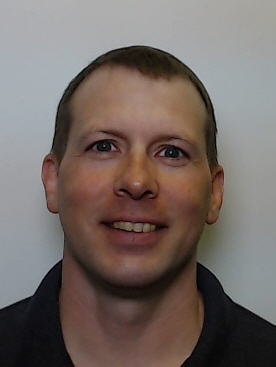
\includegraphics[width=0.25\textwidth]{figures/jva-headshop.jpeg}
  \end{center}
\end{wrapfigure}
\textbf{Jeremy Van Antwerp} earned a Ph.D.\ in chemical engineering from 
the University of Illinois at Urbana-Champaign.
More text here.
More text here.
More text here.
More text here.
More text here.
More text here.
More text here.
More text here.
More text here.
More text here.
More text here.
More text here.
More text here.
More text here.
More text here.
More text here.
More text here.
More text here.
More text here.
More text here.
More text here.
More text here.
More text here.
More text here.
More text here.
More text here.
More text here.
More text here.
More text here.
More text here.
More text here.
More text here.
More text here.
More text here.
More text here.
More text here.
More text here.
More text here.
More text here.
More text here.
More text here.
More text here.
More text here.
More text here.
More text here.
More text here.
More text here.
More text here.
More text here.


\section*{Matthew Kuperus Heun}

% Adjust spacing so the photo looks nice in the paragraph.
\setlength{\intextsep}{-7pt}%
\setlength{\columnsep}{8pt}%
\begin{wrapfigure}{L}{0.25\textwidth}
  \begin{center}
    \includegraphics[width=0.25\textwidth]{figures/Heun-pub-photo-headshot}
  \end{center}
\end{wrapfigure}
\textbf{Matthew Kuperus Heun} is Professor of Engineering 
(mechanical concentration)
at Calvin College in Grand Rapids, MI, USA.
He earned an M.S.\ and Ph.D.\ in mechanical engineering from 
the University of Illinois at Urbana-Champaign and 
later worked at NASA's Jet Propulsion Laboratory and at Global Aerospace Corporation. 
He has been a visiting scholar at the Centre for Renewable and Sustainable Energy Studies 
at the University of Stellenbosch, South Africa. 
His long-term research question is 
``What is the relationship between energy and the economy when viewed through the lens of sustainability?''
In addition to scores of articles, he is lead author of 
\emph{Beyond GDP: National accounting in the age of resource depletion}~\citep{Heun:2015aa} 
and a co-editor of
\emph{Beyond Stewardship: New approaches to creation care}~\citep{Warners:2019aa}.
                 % author(s)'s short bio(s)
								% please see the bios folder for some pdf examples

%   
% please use TexLive 2014 or later with the M&C macros freely
% available from tug.org or use any other recent version of LaTeX

\documentclass{book}

%the main style; default LibreCaslon font
\usepackage[raggedsec]{morgan2}
\usepackage{morgan-defs}

%to use Times New Roman, instead of LibreCaslon, please uncomment the next line
%\morgansetup{fontsetup=times}

% bibliography
\usepackage[square,comma,sort]{natbib}         % author-year
%usepackage[square,comma,sort,numbers]{natbib} % numbered

\setcounter{secnumdepth}{2}

\graphicspath{{./figures/}}     % folder for the figures in your book

\PassOptionsToPackage{hyphens}{url}
\usepackage[colorlinks=true,linkcolor=MyDarkBlue,
citecolor=MyDarkBlue,filecolor=MyDarkBlue,urlcolor=MyDarkBlue]{hyperref}

\renewcommand{\UrlBreaks}{\do\.\do\@\do\\\do\/\do\!\do\_\do\|\do\;\do\>\do\]%
\do\)\do\,\do\?\do\&\do\'\do+\do\=\do\#%
\do\a\do\b\do\c\do\d\do\e\do\f\do\g\do\h\do\i\do\j%
\do\k\do\l\do\m\do\n\do\o\do\p\do\q\do\r\do\s\do\t%
\do\u\do\v\do\w\do\x\do\y\do\z\do\A\do\B\do\C\do\D%
\do\E\do\F\do\G\do\H\do\I\do\J\do\K\do\L\do\M\do\N%
\do\O\do\P\do\Q\do\R\do\S\do\T\do\U\do\V\do\W\do\X%
\do\Y\do\Z}
\makeatletter
\g@addto@macro{\UrlBreaks}{\UrlOrds}
\renewcommand{\ALG@name}{\color{black}Algorithm}
\makeatother

% Begin packages imported by the authors.
\usepackage{wrapfig}  % To wrap text around figures.



%\makeindex                     % if you are creating an index for your book

\begin{document}

 \frontmatter                   % we'll produce the fm for you; 
    
\def\HALFTITLE{The Multifaceted Nature\\
			of Sustainability Challenges:\\
			An Engineering Perspective}
\def\TITLE{The Multifaceted Nature of Sustainability Challenges}
\def\AUTHORA{Jeremy Van Antwerp}
\def\AFFILIATIONA{Engineering Department, Calvin College}
\def\AUTHORB{Matthew Kuperus Heun}
\def\AFFILIATIONB{Engineering Department, Calvin College}
\def\AUTHORS{\AUTHORA\ and \AUTHORB}
\def\LECTURE{\ \#13}
\def\lcSYNTHESIS{Synthesis Lectures on XYZ}
\def\SYNTHESIS{\MakeUppercase{\textit{\lcSYNTHESIS}}}

\def\EDITOR{xxxx, \textit{yyyy}}


%%%%%%%%%%%% HALF TITLE PAGE 1-2

\thispagestyle{emptyrule}

\halftitle{\HALFTITLE}

\clearpage


%%%%%%%%%%%% FULL TITLE 5

\blankpage

\thispagestyle{emptyrule}
\title{\TITLE}

\vspace*{2pc}
\authorname{\AUTHORA}
\authoraffiliation{\AFFILIATIONA}

\vspace*{1pc}
\authorname{\AUTHORB}
\authoraffiliation{\AFFILIATIONB}

\vfill
\synthesis{\SYNTHESIS\LECTURE}
\morganlogo

\clearpage


%%%%%%%%%%%% ABSTRACT AND KEYWORDS   6

\thispagestyle{emptyrule}

\ABSTRACT
\noindent
The abstract goes here. 

The Abstract and the keywords have to fit in this page.
%end ABSTRACT

\keywords{%
xxx, yyyy, zz
}

\vfill

\clearpage


%%%%%%%%%%%%% DEDICATION  7-8


%{
%\clearpage
%\thispagestyle{plain}
%
%\vspace*{13pc}\Large\it
%\centerline{To Eric, Jacob, and my parents.}
%
%}
%
%\clearpage
 

%%%%%%%%%%%%%%%%%%%%%%%% TOC %%%%%%%%%%%%%%%%%%

%blankpage

{
\pagestyle{plain}
\tableofcontents
}

\clearpage
 
 
%%%%%%%%%%%%%%%%%%%%%%%% PREFACE %%%%%%%%%%%%%%%%%%%
 
 
\blankpage

{
\chapter*{Preface}
\addcontentsline{toc}{chapter}{\protect\numberline{}{Preface}}
\thispagestyle{plain}
\markboth{PREFACE}{PREFACE}

\noindent
This is the Preface.


\vspace*{2pc}
\noindent\AUTHORS\\
\noindent December 2019
}

\clearpage


%%%%%%%%%%%%%%%%%%%%%%%% ACK %%%%%%%%%%%%%%%%%%%


\blankpage

\chapter*{Acknowledgments}
\addcontentsline{toc}{chapter}{\protect\numberline{}{Acknowledgments}}
\thispagestyle{plain}
\markboth{ACKNOWLEDGMENTS}{ACKNOWLEDGMENTS}

\noindent
This the Acknowledgments' page.

\vspace*{2pc}
\noindent\AUTHORS\\
\noindent December 2019
 
\clearpage

\blankpage

                  % we'll need an Abstract and Keywords
								% please see the abs-pref folder for some pdf examples

 \mainmatter                    % sample chapters
    
\chapter{Information Theory and Rate Distortion Theory}
\label{ch01}


Please see below examples of equations using \verb+\begin{equation}+ \ldots
\verb+\end{equation}+ and \verb+align+.

The M\&C macros support various environments like:
constraint, construction, 
convention, conventions, corollary, definition, dictionary,
example, lemma, note, notation, observation, property, proposition,
remark, rules, theorem, etc.

What if you need an environment that the macros do not provide,
like ``guesswork?'' You create it with \verb+newMCtheorem+:

\verb+newMCtheorem}{guesswork}{GuessWork}+

\newMCtheorem{guesswork}{GuessWork}

\noindent
and use then use it:
\begin{guesswork}
This is pure guess work.
\end{guesswork}


\section{Introduction}
\label{ch01.sec1}

Thus far in the book, the term \textit{information}
\index{information}%
has been used sparingly and when
it has been used, we have purposely been imprecise as to its meaning.

\begin{figure}[hbt] % 01
\centering
  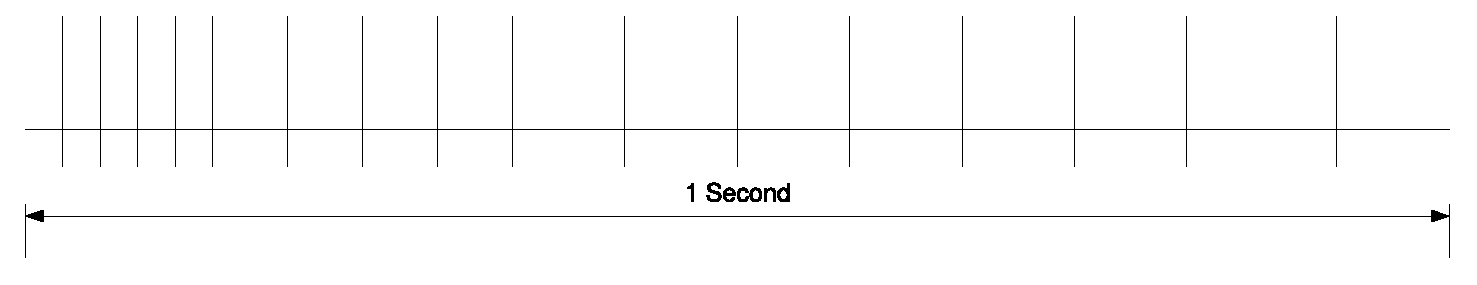
\includegraphics[width=3.3in]{line-spaces.eps}
\caption{Communication system block diagram.}
\label{ch01.fig1} 
\end{figure}

\begin{figure}[hbt] % 01
\centering
  \figboxes
\caption{Communication system block diagram.}
\label{ch01.fig2} 
\end{figure}

Examples of side-by-side figures.

%  F 2
\begin{figure}[hbt]%
\centering
\begin{subfigure}[t]{0.45\textwidth}%
	\smfigboxes
\caption{Annotated visualization of the structure of a biological neuron, reconstructed from electron microscope images of 30nm-thick slices of a mouse 
brain~\cite{tesniere59}.}%
\label{fig:bioneuron}%
\end{subfigure}%
\qquad%
\begin{subfigure}[t]{0.45\textwidth}%
	\smfigboxes
\caption{The shape of an action potential. A small external voltage stimulus (blue) triggers a cascade of charge build-up inside a neuron (red) via voltage-gated ion channels. The activation threshold is shown as a dotted line. Simulated using a Hodgkin-Huxley model of a neuron~\protect\cite{weber-97}.}%
\label{fig:ap}%
\end{subfigure}%
\caption{The structure and operation of biological neurons.}%
\end{figure}

%  F 3
\begin{figure}[b]
\centering
\begin{subfigure}[t]{0.45\textwidth}
	\smfigboxes
\caption{Points in $\mathbb{R}^2$, subdivided by a single linear classifier. One simple way of understanding linear classifiers is as a line (or hyper-plane, in higher dimensions) which splits space into two regions. In this example, points above the line are mapped to class 1 (red); those below, to class 0 (blue).}
\label{subfig:linclass}
\end{subfigure}%
\qquad%
\begin{subfigure}[t]{0.45\textwidth}
	\smfigboxes
\caption{Points in $\mathbb{R}^2$, subdivided by a combination of four linear classifiers. Each classifier maps \emph{all} points to class 0 or 1, and an additional linear classifier is used to combine the four. This hierarchical model is strictly more expressive than any linear classifier by itself.}
\label{subfig:circclass}
\end{subfigure}%
\caption{Simple elements can be combined to express more complex relationships.
This is one basic tenet of deep neural networks.}
\label{fig:classifiers}
\end{figure}


\section{Entropy and Average Mutual Information}
\label{ch01.sec2}

Consider a discrete random variable $U$ that takes on
the values $\{u_1, u_2, \dots, u_M\}$, where the set of possible
values of $U$ is often called the \textit{alphabet} and the elements
of the set are called \textit{letters} of the alphabet. Let $P_U(u)$
denote the probability  assignment  over the alphabet, then we can
define the \textit{self-information} of the event $ u = u_j $ by
\begin{equation}
  I_U \left( u_j \right) = \log \frac{1}{P_U (u_j)} = - \log P_U
    \left( u_j \right).
\label{ch01.eq1}
\end{equation}

\begin{example}
\label{ch01.ex1}
Given a random variable $U$ with four equally likely letters
in its alphabet, we wish to find $H(U)$. Clearly, $M=4$
and $P_U(u_i)= \tfrac{1}{4}$ for $ i = 1, 2, 3, 4 $.

\begin{align}
    I_{W;X}\left(w_j;x_k\right)
    & = \log
    \frac{P_{WX}\left(w_j, x_k\right)}{P_W\left(w_j\right)
              P_X\left(x_k\right)}
    \notag\\
    & = \log
    \frac{P_{X|W} \left( x_k | w_j\right)} {P_X \left(x_k\right)}
    =
     I_{X;W} \left(x_k; w_j\right).
\label{ch01.eq2}
\end{align}
\end{example}

\begin{property}
\label{ch01.pro1}
Let $U$ be a random variable with possible values $\{u_1,u_2,\dots, u_M\}$.
\end{property}

Example~\ref{ch01.ex1} illustrates Property~\ref{ch01.pro1}.

\begin{property}
\label{ch01.pro2}
Let $W$ and $X$ be jointly distributed random variables.
\end{property}

\begin{example}
\label{ch01.ex2}
Here we wish to calculate the mutual information and the average
mutual information for the probability assignments
(with $M=2$ and $N=2$)
\begin{equation}
 P_W \big(w_1\big) = P_W \big(w_2\big) = \tfrac{1}{2}
\label{ch01.eq3}
\end{equation}
\end{example}

\begin{example}[\cite{Boeringer}]
\label{ch01.ex3}
The source output is a ternary-valued random variable that takes on the
values $\{ u_1, u_2, u_3 \}$ with probabilities
$P(u_1) = 0.7, P(u_2) = 0.15 = P(u_3)$. 
\end{example}

\begin{theorem}[(Source Coding Theorem).]
\label{ch01.th1}
For a DMS with entropy $H(U)$,
the minimum average codeword length per source letter $(\bar{n})$ for any
code is lower
bounded by $H(U)$, that is, $\bar{n} \geq H(U)$, and further, $\bar{n}$
can be made as close to $H(U)$
as desired for some suitably chosen code.
\end{theorem}

\begin{theorem}[(Channel Coding Theorem~\cite{Wen-ChungLiu2005}).]
\label{ch01.th2}
Given a DMS
with entropy $H$ bits/source letter and a DMC with capacity $C$
bits/source letter,
if $H \leq C$, the source output can be encoded for transmission over
the channel with
an arbitrarily small bit error probability. Further, if $H > C$, the bit error
probability is bounded away from $0$.
\end{theorem}

\begin{proof}
This result can be proved in several ways, including calculus of
variations~\cite{WenWangetal2005} inequality; however, an
alternative method is used here.
\end{proof}

\begin{table}[hbt]
\caption{Timer0 Compare Output Mode, non-PWM Mode}
\label{ch01.tab1} 
\begin{center}
\begin{tabular}{|c|l|}
    \cb COM0x1-0
  & \cb Description 
\\
    \cw 00
  & \cw Normal port operation
\\
    \cy 01
  & \cy Toggle on Compare Match
\\
    \cw 10
  & \cw Clear on Compare Match
\\
    \cy 11
  & \cy Set on Compare Match
\\
\hline
\end{tabular}
\end{center}
\end{table}


\begin{center}
\begin{tabular}{|cl|}
    \cb COM0x1-0
  & \cb Description 
\\
    \cw 00
  & \cw Normal port operation
\\
    \cy 01
  & \cy Toggle on Compare Match
\\
    \cw 10
  & \cw Clear on Compare Match
\\
    \cy 11
  & \cy Set on Compare Match
\\
\hline
\end{tabular}
\end{center}


\section*{Summary}

In this chapter we have discussed very briefly some of the salient
results from information theory and rate distortion theory and have
indicated how these results can be used to bound communication system
performance.


\section*{Problems}
\index{problems}%

\begin{problems}

\item
A random variable $U$ has a sample space consisting of the set
of all possible binary sequences of length $N$, denoted
$\{u_j, j=1, 2, \ldots, 2^N \}$.

\item
Given a random variable $U$ with the alphabet $\{ u_1, u_2, u_3, u_4 \}$
and probability assignments $P(u_1) = 0.8, P(u_2)=0.1$,
$P(u_3) = 0.05, P(u_4)=0.05$, calculate the entropy of $U$.
Compare your result to a random variable with equally likely values.

\end{problems}

\clearpage

                % various environments like theorem,
    
%blankpage

\chapter{Jordan Canonical Form}
\label{ch02}
\index{jordan canonical form@Jordan Canonical Form}%

\section{The Diagonalizable Case}

Although, for simplicity, most of our examples
will be over the real numbers
(and indeed over the rational numbers), we will consider that
\textit{all of our vectors and matrices
are defined over the complex numbers} $\mathbb{C}$.
It is only with this assumption that the
theory of Jordan Canonical Form (JCF) works
\index{jcf@JCF}%
completely.
See Remark~\ref{ch02.rem1} for the key reason why.

\begin{definition}
\label{ch02.def1}
If \(v \neq 0\) is a vector such that, for some
$\lambda$,
\[
A v = \lambda v,
\]
then $v$ is an \textit{eigenvector} of $A$ associated
\index{eigenvector}%
to the \textit{eigenvalue} $\lambda$.
\index{eigenvalue}%
\end{definition}

\begin{example}
\label{ch02.ex1}
Let $A$ be the matrix $A =$
Then, as you can check, if $v_1 =$ 
then $A v_1 = 3 v_1$, so $v_1$ is an eigenvector of $A$ with associated
eigenvalue $3$, and if $v_2 =$ 
then $A v_2 = -2 v_2$, so $v_2$ is
an eigenvector of $A$ with associated eigenvalue $-2$.
\end{example}

\begin{remark}
\label{ch02.rem1}
This is the customary definition of the characteristic
\index{characteristic polynomial}%
polynomial.
But note that, if $A$ is an $n$-by-$n$ matrix, then the matrix
$\lambda I - A$ is obtained from the matrix $A - \lambda I$ by multiplying
each of its $n$ rows by $-1$, and hence
In practice, it is most convenient
to work with $A -\lambda I$ in finding eigenvectors---this minimizes
arithmetic---and when we come to find
chains of generalized eigenvectors in
Section~1.2,
it is (almost) essential to use $A -\lambda I$, as using
$\lambda I - A$ would introduce lots of spurious minus signs.
\end{remark}

\clearpage

                % example, etc.
    
%blankpage

\chapter{An Algorithm}
\label{ch03}

The navigation oriented heuristic ($h3$) considers the site topology.
Accesses to cached pages are not recorded in the
Web log due to the browser or proxy cache.
Therefore, references to those pages are missed.
The missing references in the log file can be found using a set of
assumptions.
The referrer field of the Web log or the Web site structure can be used
to infer cached pages.
If a requested Web page $p_i$ is not reachable
from previously visited pages in a
session, then a new session is constructed starting with page $p_i$.

\begin{algorithm}
\hrulefill

 \textit{Input :} Web server logs \newline
 \textit {Output :} set of user sessions
$\mathcal{S}=\{s_{1},...,s_{M}\}$

\hrulefill

\begin{algorithmic}[1]
 \STATE $\mathcal{S}=\{\emptyset\}$
 \STATE Order all Web logs by user IDs ($u_k$) and time increasingly
 \FORALL {user ID $u_k$}
    \STATE Create a new user session in $\mathcal{S}$ for user $u_k$
    \FOR {i=1 to the number of records of this $u_k$}
    	\IF {$t_{i+1} - t_i < \triangle t$}
    		\STATE insert this record into user session
    	\ELSE
    		\STATE Create a new user session in $\mathcal{S}$ for user $u_k$
    	\ENDIF
    \ENDFOR
 \ENDFOR
\end{algorithmic}
\hrulefill
 \caption{Construction of user sessions from Web server logs using $h1$
 heuristic}
\label{alg:visitingTimeAlg}
\end{algorithm}

\clearpage

                % algorithm sample
    
%blankpage

\chapter{Shaded Areas}
\label{ch04}

M\&C provides a macro called \verb+mcframe+ that allows us to
create a frame around some text which automatically breaks its contents
across pages. 

\verb+\begin{mcframe}[width](text-width)<background-color>+\\

\ldots

\verb+\end{mcframe}+

The optional arguments are:
\begin{itemize}
\item
\verb+width+ defaults to the width of the page
\item
\verb+text-width+ defaults to an indent of 10pt in each margin
\item
\verb+background-color+ defaults to the \verb+bluetwenty+ color of the
	M\&C books.
\end{itemize}

\blankline
Here are a few examples using some text from the book \textit{General Game 
Playing} by M. Genesereth and M. Thielscher that was published by M\&C in 
March, 2014:

\begin{mcframe}
\verb+\begin{mcframe}+\\
Games of strategy, such as Chess, couple intellectual activity with
competition.
We can exercise and improve our intellectual skills by playing such games.
The competition adds excitement and allows us to
compare our skills to those of others.
The same motivation accounts for
interest in Computer Game Playing as a testbed for Artificial Intelligence.
Programs that think better should be able to win more
games, and so we can use competitions as an evaluation technique for
intelligent systems.

Unfortunately, building programs to play specific games has limited
value in AI.  (1)~To begin with, specialized game players are very narrow.
They can be good at one game but not another. Deep Blue may have beaten
the world Chess champion, but it has no clue how to play checkers.  (2)~A
second problem with specialized game playing systems is that they do only
part of the work. Most of the interesting analysis and design is done in
advance by their programmers. The systems themselves might as well be
tele-operated.

All is not lost. The idea of game playing can be used to good effect
to inspire and evaluate good work in Artificial Intelligence, but it
requires moving more of the design work to the computer itself.
This can be done by focussing attention on General Game Playing.\\
\verb+\end{mcframe}+
\end{mcframe}

\begin{mcframe}[.7\textwidth](.6\textwidth)
\verb+\begin{mcframe}[.7\textwidth](.6\textwidth)+\\
Games of strategy, such as Chess, couple intellectual activity with
competition.
We can exercise and improve our intellectual skills by playing such games.
The competition adds excitement and allows us to
compare our skills to those of others.
The same motivation accounts for
interest in Computer Game Playing as a testbed for Artificial Intelligence.
Programs that think better should be able to win more
games, and so we can use competitions as an evaluation technique for
intelligent systems.

Unfortunately, building programs to play specific games has limited
value in AI.  (1)~To begin with, specialized game players are very narrow.
They can be good at one game but not another. Deep Blue may have beaten
the world Chess champion, but it has no clue how to play checkers.  (2)~A
second problem with specialized game playing systems is that they do only
part of the work. Most of the interesting analysis and design is done in
advance by their programmers. The systems themselves might as well be
tele-operated.\\
\verb+\end{mcframe}+
\end{mcframe}

\begin{mcframe}[.8\textwidth](.7\textwidth)<green>
\verb+\begin{mcframe}[.8\textwidth](.7\textwidth)<green>+\\
Games of strategy, such as Chess, couple intellectual activity with
competition.
We can exercise and improve our intellectual skills by playing such games.
The competition adds excitement and allows us to
compare our skills to those of others.
The same motivation accounts for
interest in Computer Game Playing as a testbed for Artificial Intelligence.
Programs that think better should be able to win more
games, and so we can use competitions as an evaluation technique for
intelligent systems.

Unfortunately, building programs to play specific games has limited
value in AI.  (1)~To begin with, specialized game players are very narrow.
They can be good at one game but not another. Deep Blue may have beaten
the world Chess champion, but it has no clue how to play checkers.  (2)~A
second problem with specialized game playing systems is that they do only
part of the work. Most of the interesting analysis and design is done in
advance by their programmers. The systems themselves might as well be
tele-operated.\\
\verb+\end{mcframe}+
\end{mcframe}

\clearpage

                % shaded blocks in your pages
    
%blankpage

\chapter{Math}
\label{ch05}

\section{Bold Math}
Sometimes you have a math symbol in bold to indicate, for example,
a vector or special functions. Use \verb+\mathbf{x}+ for letters
and \verb+\bm{\Phi}+ for Greek letters.

\noindent
\ldots
$\bm{\Phi}$ and $\bm{\Theta}$ are the distribution functions
governing the likelihood of $\mathcal{X}$ and $\mathbf{Z}$ \ldots

\blankline
Some notes:
\begin{itemize}
\item
use \verb+\bm{\Phi}+ to produce a bold Greek symbol Phi.
\item
use \verb+\mathcal{X}+ to display the caligraphic letter X
\item
use \verb+\mathbf{Z}+ to dispaly bold non-Greek symbols
\end{itemize}

\blankline
If you plan to use Greek symbols to identify, for example, vectors, you could
create a macro, like

\verb+\newcommand{\vect}[1]{\bm{#1}}+

\newcommand{\vect}[1]{\bm{#1}}

and then use

\noindent
\begin{verbatim}
\ldots the vectors are $\vect{\Phi}$ and $\vect{\Theta}$ \ldots
\end{verbatim}

to produce

\noindent
\ldots the vectors are $\vect{\Phi}$ and $\vect{\Theta}$ \ldots

\blankline
The idea is to have macro names for different constructs.
If you chose to use a different representation for vectors,
you change the macro and rerun your manuscript.


\section{Math Variables}

When we have a math variable with more than one character,
like \textit{abcd}, \LaTeX{} treats each character as a separate variable.
With Caslon fonts, that we use to produce your book, that space is noticeable.

We eliminat the extra space using \verb+\mathit+:

\verb+\mathit{abcd} = 3.+
$$
\mathit{abcd} = 3.
$$

If we use the variable \textit{abcd} often, as in

\verb|\mathit{abcd} = \mathit{abcd}^2 - \sqrt{\mathit{abcd}} + \mathit{abcd},|

$$
\mathit{abcd} = \mathit{abcd}^2 - \sqrt{\mathit{abcd}} + \mathit{abcd},
$$
we can create a separate macro for the variable:

\verb+\newcommand{\abcd}{\mathit{abcd}}+
\newcommand{\abcd}{\mathit{abcd}}

\noindent
Then we can use \verb+\abcd+ in the expressions:

\verb|\abcd = \abcd^2 - \sqrt{\abcd} + \abcd,|

$$
\abcd = \abcd^2 - \sqrt{\abcd} + \abcd,
$$

If there is already a predefined command with the same name,
we use instead something like \verb+Abcd+:

\verb+\newcommand{\Abcd}{\mathit{abcd}}+
\newcommand{\Abcd}{\mathit{abcd}}

\noindent
Then we can use \verb+\Abcd+ in the expressions:

\verb|\Abcd = \Abcd^2 - \sqrt{\Abcd} + \Abcd.|

$$
\Abcd = \Abcd^2 - \sqrt{\Abcd} + \Abcd.
$$


\clearpage

                % bold math and math variables
    
%blankpage

\chapter{Citations with Author-Year}
\label{ch06}

An alternative to numerical \LaTeX\ citations makes reference to published
works by citing the author's name and year of publication. The entries in 
the bibliographic listing are not numbered. The citation itself may be 
either parenthetical like \citep{carroll98} or textual as shown by
\citet{carroll98}.

The \verb+natbib+ package by Patrick W. Daly is the most universal package
for Author-Year citation and it is compatible with \verb+\bibitem+ syntaxes
and with the \verb+.bst+ files of author-year packages such as
\verb+apalike+, \verb+chicago+, and \verb+harvard+.

If you create a bibliography by hand, please see the file \verb+biblio.tex+
in the \verb+latex+ directory of \verb+bib-AY.zip+.
The \verb+biblio.tex+ files shows the syntax that \verb+natbib.sty+ 
requires and notice how we use
that package in~\verb+book.tex+ and in~\verb+ch01.tex+. 
You can find the details about \verb+natbib+ and Author-Year bibliographies
in~\citet[pages~218-221]{KD:2004}.

Note that we have bibliographic references like \verb+carroll98+,
\verb+KD:2004+, and \verb+weber-97+. Pick a style that works for you
and stay with it, then it will be easier for yourself and others to 
maintain and modify your bibliography and citations.

If you use \verb+.bib+ files then you should know about \verb+BibTeX+,
\verb+.bst+ files, and you should know how to create the \verb+.bbl+
files as well.
(If you use \verb+.bib+ files but you do not know the rest, you should
consult a local expert before continuing with \verb+.bib+ or create
your bibliography by hand.)
If you know the steps we mentioned above and you wish to create an 
Author-Year bibliography and citations, then you are in luck: 
there are three \verb+.bst+ that are provided with \verb+natbib+.
They are: \verb+plainnat+, \verb+unsrtnat+, and \verb+abbrvnat+.

Once you create your \verb+.bbl+ file(s), please submit them along with
your manuscript files, style files, and (preferably) \verb+.eps+ figures with 
\verb+BoundingBox+es to \textit{Morgan and Claypool Publishers.}

You can get a free copy of the \verb+natbib+ package  from CTAN at
\begin{center}
\verb+http://www.ctan.org/tex-archive/macros/latex/contrib/natbib/+
\end{center}
and download the file \verb+natbib.zip+.

Here are some more samples using the citations that appear in the file
\verb+biblio.tex+ that we built by hand.

The next paragraph uses text citations using \verb+\citet+ (cite as text):\\
\noindent
There are several textbooks that give a general 
introduction to dependency grammar but
most of them in other languages than English, for example,
\citet{tarvainen82} and~\citet{weber-97}.

The last paragraph uses text citations with parentheses
using \verb+\citetp+:\\
\noindent
Tesni{\`e}re's seminal work was published
posthumously as~\citep{tesniere59}. 
Other influential theories in the dependency
grammar tradition include Functional Generative
Description~\citep{SHP:1986}.

Please see the bibliography on the next page and the file \verb+biblio.tex+.

\clearpage

                % bibliography using Author-Year

    
\blankpage

\begin{thebibliography}{xx}
\addcontentsline{toc}{chapter}{\protect\numberline{}{Bibliography}}
\markboth{BIBLIOGRAPHY}{BIBLIOGRAPHY}

\bibitem[Boeringer and Werner(2004)D. Boeringer and D. Werner]{Boeringer}
D. Boeringer and D. Werner,
``Particle swarm optimization versus genetic algorithms for
phased array synthesis,''
\textit{IEEE Trans. Antennas Propagat.,}
vol.~52, no.~3, pp.~771--779, 2004.

\bibitem[Carroll et~al.(1998)Carroll, Briscoe, and Sanfilippo]{carroll98}
Carroll, John, Briscoe, Edward, and Sanfilippo, Antonio
Supertagging: An approach to almost parsing,
\textit{Computational Linguistics} 25(2):237--267.

\bibitem[Ho et al(2005)Ho et al]{Hoetal2005}
S. Ho, S. Yang, G. Ni, E. W. C. Lo, and H. C. Wong,
``A particle swarm optimization-based method for multiobjective
design optimizations,''
\textit{IEEE Trans. Magn.},
vol.~41, no.~5, pp.~1756--1759, 2005.

\bibitem[Kopka and Daly(2004)W. Kopka and P.W. Daly]{KD:2004}
Kopka, Helmut and Daly, Patrick W. 
\textit{Guide to \LaTeX,} fourth edition, Addison Wesley.

\bibitem[Levin (2002)F.S. Levin]{Levin2002}
F. S. Levin,
\textit{An Introduction to Quantum Theory},
Cambridge: Cambridge University Press, 2002.

\bibitem[Liu (2005)W.-C. Liu]{Wen-ChungLiu2005}
W-C Liu,
``A design of a multiband
CPW-fed monopole antenna using a particle swarm optimization approach,''
\textit{IEEE Trans. Antennas Propagat.,}
vol.~53, no.~10, pp.~3273--3279, 2005.

\bibitem[Sgall et~al.(1986)Sgall, Haji\v{c}ov\'{a}, and Panevov\'{a}]
{SHP:1986}
Sgall, Petr, Haji\v{c}ov\'{a}, Eva, and Panevov\'{a}, Jarmila.
\textit{The Meaning of the Sentence in Its Pragmatic Aspects}, Reidel.

\bibitem[Tarvainen (1982)Tarvainen]{tarvainen82}
Tarvainen, Kalevi.  
\textit{Einf\"{u}hrung in die {D}ependenzgrammatik}, Niemeyer.

\bibitem[Tesni{\`e}re (1959)Tesni{\`e}re]{tesniere59}
Tesni{\`e}re, Lucien.  
\textit{\'El\'ements de syntaxe structurale}, Editions Klincksieck.

\bibitem[Weber (1997)Weber, H.J.]{weber-97}
Weber, H.~J. 
\textit{Dependenzgrammatik.\ Ein interaktives Arbeitsbuch},
G\"unter Narr.

\bibitem[Wang et al(2005)W. Wang et al]{WenWangetal2005}
W. Wang, Y. Lu, J. S. Fu, and Y. Z. Xiong,
``Particle swarm optimization and finite-element based
approach for microwave filter design,''
\textit{IEEE Trans. Magn.},
vol.~41, no.~5, pp.~1800--1803, 2005.

\end{thebibliography}

\clearpage

              % bibliography

 \backmatter                    % back matter
    
%blankpage

\chapter*{Author's Biography}
\markboth{AUTHOR'S BIOGRAPHY}{AUTHOR'S BIOGRAPHY}
\addcontentsline{toc}{chapter}{\protect\numberline{}{Author's Biography}}


\section*{Jeremy Van Antwerp}

% Adjust spacing so the photo looks nice in the paragraph.
\setlength{\intextsep}{-7pt}%
\setlength{\columnsep}{8pt}%
\begin{wrapfigure}{L}{0.25\textwidth}
  \begin{center}
    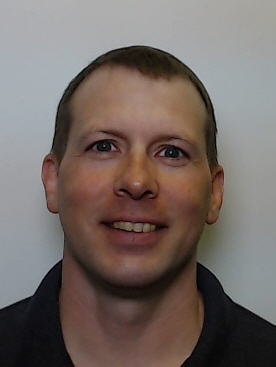
\includegraphics[width=0.25\textwidth]{figures/jva-headshop.jpeg}
  \end{center}
\end{wrapfigure}
\textbf{Jeremy Van Antwerp} earned a Ph.D.\ in chemical engineering from 
the University of Illinois at Urbana-Champaign.
More text here.
More text here.
More text here.
More text here.
More text here.
More text here.
More text here.
More text here.
More text here.
More text here.
More text here.
More text here.
More text here.
More text here.
More text here.
More text here.
More text here.
More text here.
More text here.
More text here.
More text here.
More text here.
More text here.
More text here.
More text here.
More text here.
More text here.
More text here.
More text here.
More text here.
More text here.
More text here.
More text here.
More text here.
More text here.
More text here.
More text here.
More text here.
More text here.
More text here.
More text here.
More text here.
More text here.
More text here.
More text here.
More text here.
More text here.
More text here.
More text here.


\section*{Matthew Kuperus Heun}

% Adjust spacing so the photo looks nice in the paragraph.
\setlength{\intextsep}{-7pt}%
\setlength{\columnsep}{8pt}%
\begin{wrapfigure}{L}{0.25\textwidth}
  \begin{center}
    \includegraphics[width=0.25\textwidth]{figures/Heun-pub-photo-headshot}
  \end{center}
\end{wrapfigure}
\textbf{Matthew Kuperus Heun} is Professor of Engineering 
(mechanical concentration)
at Calvin College in Grand Rapids, MI, USA.
He earned an M.S.\ and Ph.D.\ in mechanical engineering from 
the University of Illinois at Urbana-Champaign and 
later worked at NASA's Jet Propulsion Laboratory and at Global Aerospace Corporation. 
He has been a visiting scholar at the Centre for Renewable and Sustainable Energy Studies 
at the University of Stellenbosch, South Africa. 
His long-term research question is 
``What is the relationship between energy and the economy when viewed through the lens of sustainability?''
In addition to scores of articles, he is lead author of 
\emph{Beyond GDP: National accounting in the age of resource depletion}~\citep{Heun:2015aa} 
and a co-editor of
\emph{Beyond Stewardship: New approaches to creation care}~\citep{Warners:2019aa}.
                 % author(s)'s short bio(s)
								% please see the bios folder for some pdf examples

%   
% please use TexLive 2014 or later with the M&C macros freely
% available from tug.org or use any other recent version of LaTeX

\documentclass{book}

%the main style; default LibreCaslon font
\usepackage[raggedsec]{morgan2}
\usepackage{morgan-defs}

%to use Times New Roman, instead of LibreCaslon, please uncomment the next line
%\morgansetup{fontsetup=times}

% bibliography
\usepackage[square,comma,sort]{natbib}         % author-year
%usepackage[square,comma,sort,numbers]{natbib} % numbered

\setcounter{secnumdepth}{2}

\graphicspath{{./figures/}}     % folder for the figures in your book

\PassOptionsToPackage{hyphens}{url}
\usepackage[colorlinks=true,linkcolor=MyDarkBlue,
citecolor=MyDarkBlue,filecolor=MyDarkBlue,urlcolor=MyDarkBlue]{hyperref}

\renewcommand{\UrlBreaks}{\do\.\do\@\do\\\do\/\do\!\do\_\do\|\do\;\do\>\do\]%
\do\)\do\,\do\?\do\&\do\'\do+\do\=\do\#%
\do\a\do\b\do\c\do\d\do\e\do\f\do\g\do\h\do\i\do\j%
\do\k\do\l\do\m\do\n\do\o\do\p\do\q\do\r\do\s\do\t%
\do\u\do\v\do\w\do\x\do\y\do\z\do\A\do\B\do\C\do\D%
\do\E\do\F\do\G\do\H\do\I\do\J\do\K\do\L\do\M\do\N%
\do\O\do\P\do\Q\do\R\do\S\do\T\do\U\do\V\do\W\do\X%
\do\Y\do\Z}
\makeatletter
\g@addto@macro{\UrlBreaks}{\UrlOrds}
\renewcommand{\ALG@name}{\color{black}Algorithm}
\makeatother

% Begin packages imported by the authors.
\usepackage{wrapfig}  % To wrap text around figures.



%\makeindex                     % if you are creating an index for your book

\begin{document}

 \frontmatter                   % we'll produce the fm for you; 
    \input{fm}                  % we'll need an Abstract and Keywords
								% please see the abs-pref folder for some pdf examples

 \mainmatter                    % sample chapters
    \input{ch01}                % various environments like theorem,
    \input{ch02}                % example, etc.
    \input{ch03}                % algorithm sample
    \input{ch04}                % shaded blocks in your pages
    \input{ch05}                % bold math and math variables
    \input{ch06}                % bibliography using Author-Year

    \input{biblio}              % bibliography

 \backmatter                    % back matter
    \input{bio}                 % author(s)'s short bio(s)
								% please see the bios folder for some pdf examples

%   \input{book.ind}            % if you have an Index

\end{document}

            % if you have an Index

\end{document}

            % if you have an Index

\end{document}

            % if you have an Index

\end{document}

